%\section{Probability}
%Here we outline a few rules from the theory of probability. The simplest rule of probability is that given a series of possible outcomes, the sum of the probabilities of the outcome must equal unity. This is expressed as:
%\begin{equation}\label{eqn:probsumdiscrete}
%    \sum_{i=1}^{N} p_i = 1.
%\end{equation}
%Here $p_i$ represents the probability mass function, or more simply, the probability of the \textit{$i^{th}$} outcome, given $N$ possible events. If the random variable is continuous then we simply express this as an integral:
%\begin{equation}\label{eqn:probsumcontinuous}
%    \int p \left( x \right) dx = 1.
%\end{equation}
%Where $p(x)$ represents the probability density function of a particular outcome $x$. In this chapter we will
%often divide by $1$ using Eq.~\ref{eqn:probsumcontinuous} or depend in some way on Eq.~\ref{eqn:probsumdiscrete}.
%
%Next we describe the notion of conditional probability. The probability of two events occurring is $p(A \textrm{ and } B)$:
%\begin{equation}\label{eqn:probAandprobB}
%    p\left(A\textrm{ and }B\right) \equiv p(A,B) = p(A) \, p(B|A) = p(B) \, p(A|B)
%\end{equation}
%This new term here $p(B|A)$ is to be interpreted as the probability that event B occurs given that A has occurred, and similarly, $p(A|B)$ means the probability that event A occurs given that B has occurred.
%
%Next we describe the concept of marginalization, otherwise known as integrating out nuisance parameters. Marginalization can be done via:
%\begin{equation}
%    p(A) = \int p(A \, | \, B) \, p(B) \, dB
%\end{equation}

\section{Bayesian Inference}
Within statistical inference we are interested in leveraging our uncertainty regarding hypotheses and parameters and applying them to measurments or data in the real world. We seek a way to update our prior beliefs regarding these hypotheses and parameters in a way that is consistent and coherent with the data. We begin this approach by introducting Bayes theorem:
\begin{equation} \label{eqn:BayesTheorem_basic}
     p(\mathrm{H}) \, p(\mathbf{d} \, |\, \mathrm{H})  =  p(\mathrm{H} \, | \, \mathbf{d}) p(\mathbf{d}).
\end{equation}
Here we have $p(\mathrm{H})$ which represents our prior belief about the hypothesis H. The expression $p(\mathbf{d} \, |\, \mathrm{H})$ represents the measurement of our data which is the likelihood. We use these to update our inference on the probability of hypothesis H as expressed in the posterior probability of the hypothesis given the data, $p(\mathrm{H} \, | \, \mathbf{d})$. Finally then we have $p(\mathbf{d}$, the probability of obtaining this data set. For the moment we will consider this as a normalization factor. For ease of reading we will change notation so that the prior $p(H)$ is $\pi (H)$, the likelihood $p(\mathbf{d} \, |\, \mathrm{H})$ is $\mathcal{L}(\mathbf{d} \, | \, \mathrm{H})$, the posterior distribution $p(\mathrm{H} \, | \, \mathbf{d})$ is $\mathcal{P}(\mathrm{H} \, | \, \mathbf{d})$, and the normalization factor $p(\mathbf{d})$ is $\mathcal{Z}(\mathbf{d})$ following the notation of~\cite{hobson2010bayesian}.

Within the context of parameter estimation we often construct a hypothesis H that is constructed from prior distributions on parameter values $\vec{\theta}$ that fully describe the hypothesis. In this context it is more helpful to rewrite Eq.~\ref{eqn:BayesTheorem_basic} as
\begin{equation}\label{eqn:BayesTheorem_PE}
   \mathcal{P}(\vec{\theta} \, | \, \mathbf{d}, \mathrm{H}) = \frac{\pi(\vec{\theta} \, | \, \mathrm{H} \, \mathcal{L}(\mathbf{d} \, | \vec{\theta})}
                                                                   {\mathcal{Z}(\mathbf{d} \, | \, \mathrm{H}}.
\end{equation} 
Here we have moved the posterior probability on the parameters $\vec{\theta}$ to the left hand side of the equation and the normalization constant $\mathcal{Z}(\mathbf{d} \, | \, \mathrm{H}$ to the right hand side of the equation. In the context of Eq.~\ref{eqn:BayesTheorem_PE} the normalization constant can be understood as the marginal likelihood since it marginalizes all parameters of the model H out of the likelihood~\cite{hobson2010bayesian}:
\begin{equation}\label{eqn:marg_likelihood}
    \mathcal{Z}(\mathbf{d} \, | \, \mathrm{H} = \int pi(\vec{\theta} \, | \, \mathrm{H}) \, \mathcal{L}(\mathbf{d} \, | \vec{\theta}) d\vec{\theta}.
\end{equation} 
This marginal likelihood is often called the evidence since it summarizes the goodness of fit of the prior to the data. We can compare the evidences between different hypotheses as a way to see which hypothesis' prior distribution on parameters is a better explanation of the data. In most cases this integral is virtually intractable through traditional means. For this reason it is useful to consider Eq.~\ref{eqn:marg_likelihood} as the prior-weighted average likelihood via the following expression
\begin{equation}
    \mathcal{Z}(\mathbf{d} \, \, \mathrm{H}) = \frac{\int \pi(\vec{\theta}\, | \, \mathrm{H}) \mathcal{L}(\mathbf{d} \, | \, \vec{\theta}, \mathrm{H}) d\vec{\theta}}
                                                    {\int \pi(\vec{\theta} \, | \, \mathrm{H}) d\vec{\theta}} = \langle \mathcal{L}(\mathbf{d} \, | \, \vec{\theta}, \mathrm{H})_{\pi(\vec{\theta} \, | \, \mathrm{H})}.
\end{equation}
Here $\langle \mathcal{L}(\mathbf{d} \, | \, \vec{\theta}, \mathrm{H})_{\pi(\vec{\theta} \, | \, \mathrm{H})}$ denotes taking the average of the likelihood with respect to the measure defined by the prior distribution. Therefore, the marginal likelihood could be approximated via a Monte Carlo simulation across the prior distribution where we then measure the likelihood and sum up the contributions. In practice, this too is very difficult for all but the simplest problems. In practice we often deal with the log likelihood and not the standard likelihood since it is too small to represent on a computer, therefore it is usually standard practice to consider the logarithm of the evidence as well. We will make use of the log evidence in section~\ref{sec:practical_bayes}. We would now like to compare the relative likelihood between two competeing hypotheses. 

When comparing the evidences from two competing hypotheses that analyze the same data it is possible to weigh the relative likelihood of these hypotheses via a likelihood ratio test known as the Bayes factor. For the comparison of two hypotheses, $\mathrm{H}_A$, and $\mathrm{H}_B$, the Bayes factor is defined as
\begin{equation}
    \mathcal{B}^{\mathrm{H}_A\;\;}_{\;\;\mathrm{H}_B} = \frac{\mathcal{Z}(\mathbf{d} \, \, \mathrm{H}_A)}{(\mathbf{d} \, \, \mathrm{H}_B)}
\end{equation}
The Bayes factor can be converted into a posterior odds ratio on a hypothesis via:
\begin{equation}\label{eqn:odds_ratio}
    \mathcal{O}^{\mathrm{H}_A\;\;}_{\;\;\mathrm{H}_B} = \mathcal{B}^{\mathrm{H}_A\;\;}_{\;\;\mathrm{H}_B} \times \frac{\pi(\mathrm{H}_A)}{\pi(\mathrm{H}_B)}.
\end{equation}
In this equation, $\mathcal{O}^{\mathrm{H}_A\;\;}_{\;\;\mathrm{H}_B}$ represents the posterior odds that hypothesis $\mathrm{H}_A$ is preferred over hypothesis $\mathrm{H}_B$. The ratio $\pi(\mathrm{H}_A) / \pi(\mathrm{H}_B)$ represents our prior odds ratio, that is, how much more did we believe that hypothesis $\mathrm{H}_A$  was preferred over hypothesis $\mathrm{H}_B$  before measurement. The prior odds ratio gives us a statement of what level of Bayes factor we would require before we begin to change our minds about the odds of hypothesis $\mathrm{H}_B$ being better supported in the data than hypothesis $\mathrm{H}_A$. It is considered good practice to state prior probabilities at the outset of an experiment including prior odds ratios on hypotheses~\cite{hobson2010bayesian}. Choice of prior probabilities on hypotheses are subjective but should not be considered arbitrary since they represent decisions in experimental design. An uninformative prior on each hypothesis would then set the prior odds ratio to unity.

If there are only two hypotheses being considered then an odds ratio can be converted into a probability of one hypothesis over another hypothesis through the following expression~\cite{read2006encyclopedia}:
\begin{equation}\label{eqn:probability_odds_ratio}
    p(\mathrm{H}_A) \, | \, \mathbf{d}) = \frac{\mathcal{O}^{\mathrm{H}_A\;\;}_{\;\;\mathrm{H}_B}}{1 + \mathcal{O}^{\mathrm{H}_A\;\;}_{\;\;\mathrm{H}_B}}.
\end{equation}
And the probability for the hypothesis $\mathrm{H}_B$ is given as $p(\mathrm{H}_B)) \equiv 1 - p(\mathrm{H}_A))$. In cases where there is more than one hypothesis available we set one model as the fiducial model such that all Bayes factors are calculated relative to this fiducial model. Then posterior probabilities on all models can be calculated as
\begin{equation}
    p(\mathrm{H}_i \, | \, \mathbf{d}) = \frac{\mathcal{B}^{\mathrm{H}_i}_{\mathrm{H}_{\mathrm{fiducial}}}}
                                              {\sum^{N_{models}}_{\limit j=1} \mathcal{B}^{\mathrm{H}_j}_{\mathrm{H}_{\mathrm{fiducial}}}} .
\end{equation}
As Berger writes in the Encyclopedia of Statistical Science (\cite{read2006encyclopedia}), "[w]hile Bayes factors do summarize the evidence for various hypothese or models, they are obviously not complete summaries of the information from an experiment." Berger continues to write that Bayes factors need to be contextualized within the inference on parameters for each hypothesis (and vice-versa). Berger also writes that Bayesians cannot test precise hypotheses using credible intervals as is often done in Frequentist statistics with confidence intervals, but must instead use Bayes factors. He also writes that the Bayes factors should be understood under a framework of decision analysis. This requires expertise in the field of status.

In Fig.~\ref{fig:log10odds_v_probability} we compare the odds ratio with the posterior probability for a hypothesis. When the odds ratio is unity the probability of one hypothesis versus another is $0.5$. 
\begin{figure}
  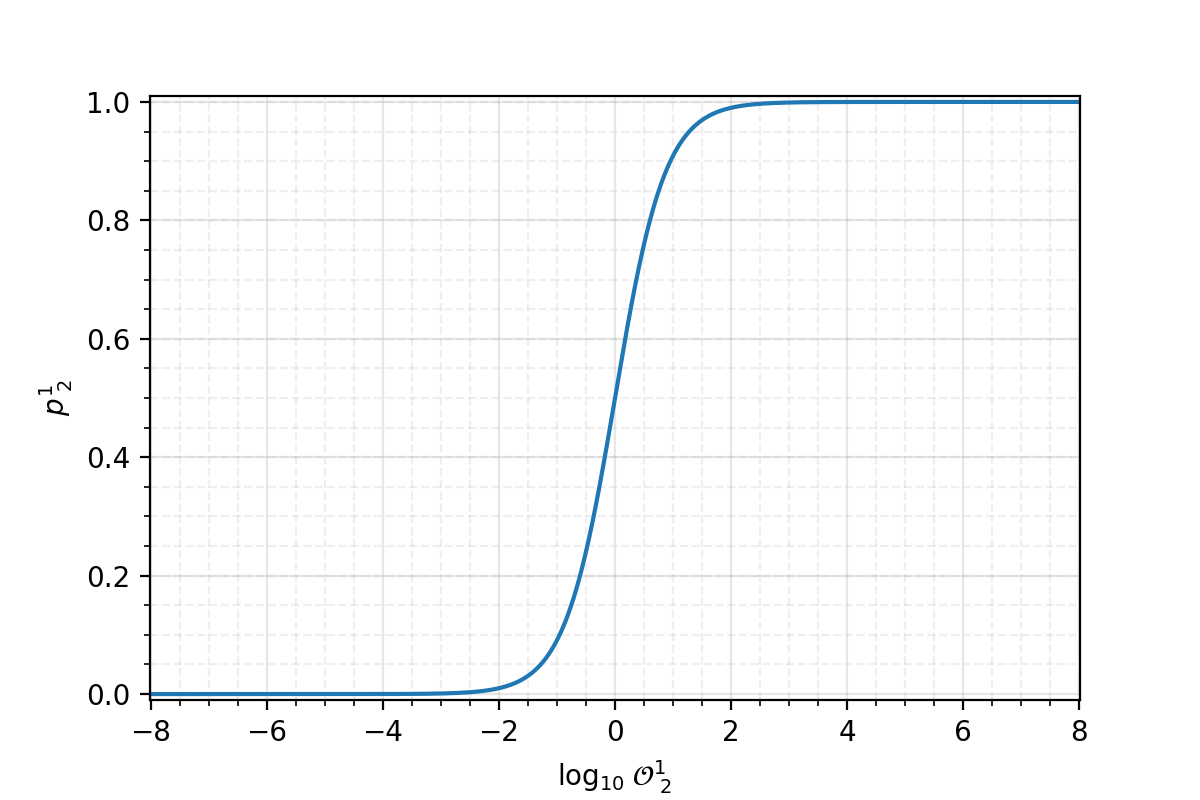
\includegraphics[width=\textwidth]{figs/chapter5/log10odds_probability.png}
  \caption{The probability of hypothesis 1 being favored over hypothesis 2 when considering the $\mathrm{log}_{10} \; \mathcal{O}$. When $\mathrm{log}_{10} \; \mathcal{O} = 0$, the probability for each hypothesis is $50\%$. At odds ratios close to 100 (0.01) the evidence becomes heavily stacked towards one hypothesis or another.}
  \label{fig:log10odds_v_probability}
\end{figure}
Furthermore, we can make a mapping of this probability to a single-tailed z-score of a Gaussian distribution. This is the familiar test statistic $\sigma$ used in physics. A z-score of $0$ ($0 \sigma$) indicates a $50\%$ probability, while a z-score of $5$ is $\sim$ $1-10^-7$ probability. Fig~\ref{fig:log10odds_v_z_score} shows how the z-score varies with odds ratio.
\begin{figure}
  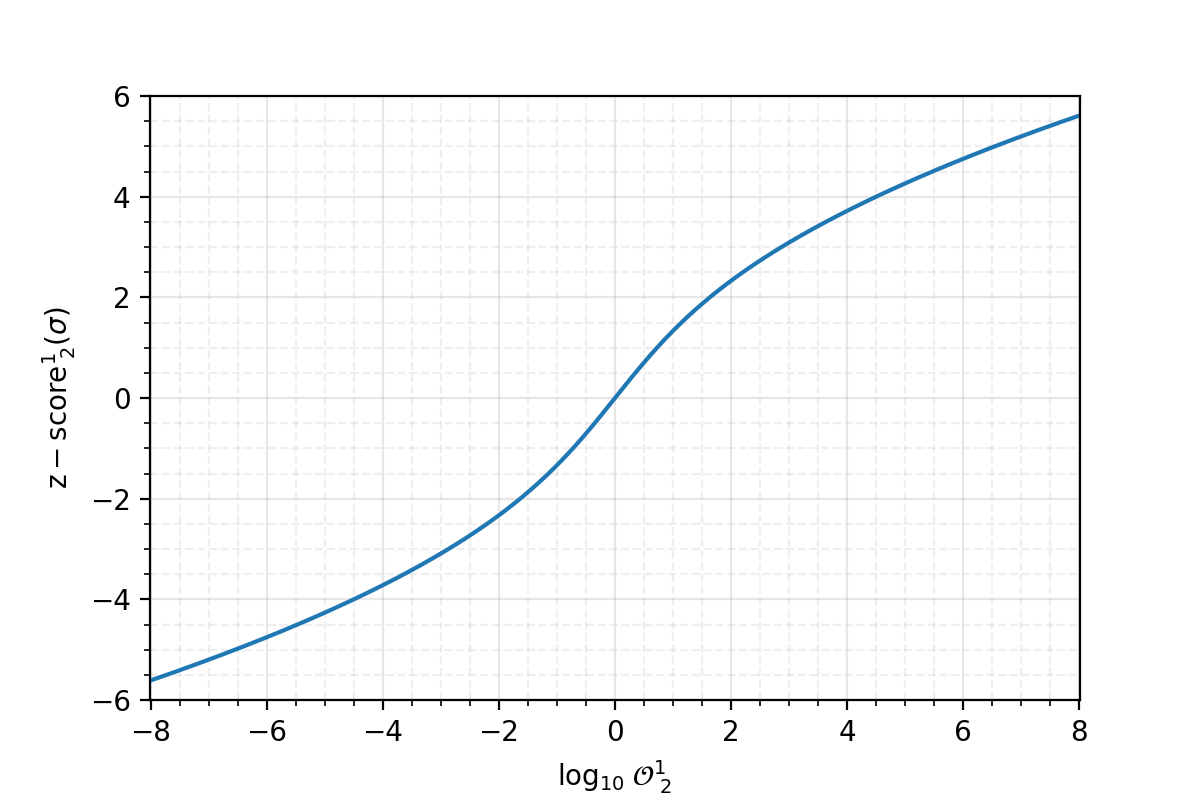
\includegraphics[width=\textwidth]{figs/chapter5/log10odds_z_score.png}
  \caption{The z-score pertaining to the same level of probability for  hypothesis 1 being favored over hypothesis 2 when considering the $\mathrm{log}_{10} \; \mathcal{O}$. When $\mathrm{log}_{10} \; \mathcal{O} = 0$, the z-score is $0 \sigma$ and the probability for each hypothesis is $50\%$. A z-score of $>5 \sigma$ has the same probability value as an odds ratio of $> 10^7$.}
  \label{fig:log10odds_v_z_score}
\end{figure}

One convenient property of odds ratios and Bayes factors is that we can multiply them over many datasets if we continue to use the same prior hypotheses on these new data. In this manner, it is possible to take low significant results from multiple experiments and gradually build evidence for a hypothesis over many experiments. We now move on towards more practical methods of estimating Bayes factors and uncertainty estimation on Bayes factors.

\section{Bayes factor estimation and uncertainty propagation}\label{sec:practical_bayes}
When comparing hypotheses practically we must confront the fact that it is impossible to calculate the evidence (or log evidence) analytically and so we often turn to Markov Chain Monte Carlo techniques to approximate the evidence~\cite{hobson2010bayesian}. These techniques will often give a point-estimate or mean value estimate of the logarithm of the evidence with some estimation of the uncertainty in the estimate. In our treatment we consider a model of the estimation of the logarithm of the evidence as a Gaussian distribution in log-likelihood. This distribution has mean $\mu_{\widehat{\mathrm{ln} \, \mathcal{Z}}}$ given by a Markov-Chain Monte Carlo (MCMC) method's point-estimate, and standard deviation $\sigma_{\widehat{\mathrm{ln} \, \mathcal{Z}}}$ representing systematic or statistical uncertainties in the MCMC method. Thus the logarithm of the evidence can be represented as 
\begin{equation}\label{eqn:p_log_z}
    p(\widehat{\mathrm{ln} \, \mathcal{Z}}) = \left(\frac{1}{\sqrt{2 \pi \sigma_{\widehat{\mathrm{ln} \, \mathcal{Z}}}}} \right) \mathrm{exp} \left \{-\frac{\left(\mathrm{ln} \, \mathcal{Z} - \mu_{\widehat{\mathrm{ln} \, \mathcal{Z}}}\right)^2} {2 \sigma_{\widehat{\mathrm{ln} \, \mathcal{Z}}}}  \right\}.
\end{equation}

Since the Bayes factor is the ratio of two evidences, the logarithm of the Bayes factor is the difference of the logarithms of two evidences,
\begin{equation}\label{eqn:log_bayes_factor}
    \mathrm{ln} \, \mathcal{B}^A_B = \mathrm{ln} \, \mathcal{Z}_{\mathrm{A}} - \mathrm{ln} \, \mathcal{Z}_{\mathrm{B}}.
\end{equation}
However, since we treat $\mathrm{ln} \, \mathcal{Z}_{\mathrm{A}}$ as a random variable we must deal with the uncertainty in $\widehat{\mathrm{ln} \, \mathcal{Z}_{\mathrm{A}}}$. The logarithm of the Bayes factor then becomes the difference between two probability distribution functions. This can be solved via convolution and has been solved for the Gaussian case~\citep{bromiley2003products}. From \cite{bromiley2003products}, we can express $\widehat{\mathrm{ln} \, \mathcal{B}^A_B}$ as a Gaussian distribution function with mean $\mu_{\widehat{\mathrm{ln} \, \mathcal{B}^A_B}} = \mu_{\widehat{\mathrm{ln} \, \mathcal{Z}_A}} - \mu_{\widehat{\mathrm{ln} \, \mathcal{Z}_B}}$ and standard deviation $\sigma_{\widehat{\mathrm{ln} \, \mathcal{B}^A_B}} = \sqrt{\sigma_{\widehat{\mathrm{ln} \, \mathcal{Z}_A}}^2 + \sigma_{\widehat{\mathrm{ln} \, \mathcal{Z}_B}}^2 }$. This gives us the following expression for the distribution function on the logarithm of the Bayes factor:
\begin{equation}\label{eqn:p_log_b}
    p(\widehat{\mathrm{ln} \, \mathcal{B}^A_B}) = \left(\frac{1}{\sqrt{2 \pi \sigma_{\widehat{\mathrm{ln} \, \mathcal{B}^A_B}}}} \right) \mathrm{exp} \left \{-\frac{\left(\widehat{\mathrm{ln} \, \mathcal{B}^A_B} - \mu_{\widehat{\mathrm{ln} \, \mathcal{B}^A_B})}\right)^2} {2 \sigma^2_{\widehat{\mathrm{ln} \, \mathcal{B}^A_B}}}  \right\}.
\end{equation}

The expression in Eq.~(\ref{eqn:p_log_b}) is a Gaussian distribution function in $\widehat{\mathrm{ln} \, \mathcal{B}^A_B}$, but we often prefer to know the estimate on $\mathcal{B}^A_B$ and so we must transform coordinates. This transformation of coordinates, is a well-known distribution called the log-normal distribution. We write out our log-normal probability distribution function for $\widehat{\mathcal{B}^A_B}$ as
\begin{equation}
    p(\widehat{\mathcal{B}^A_B}) = \frac{1}{\widehat{\mathcal{B}^A_B} \, \sigma_{\widehat{\mathrm{ln} \, \mathcal{B}^A_B}}} \frac{1}{2\pi} \mathrm{exp} \left \{-\frac{\left(\mathrm{ln} \, \widehat{\mathcal{B}^A_B} - \mu_{\widehat{\mathrm{ln} \, \mathcal{B}^A_B})}\right)^2} {2 \sigma^2_{\widehat{\mathrm{ln} \, \mathcal{B}^A_B}}}  \right\}.
\end{equation}
It is worth noting that for a sufficiently small standard deviation on the logarithm of the Bayes factor, the probability of the distribution function will look approximately Gaussian in shape. For the log-normal Bayes factor distribution the median value of the distribution is identical to the point-estimate Bayes factor, $\mathcal{B}^A_B = \mathrm{exp} \left[\mathrm{ln} \, \mathcal{Z}_{\mathrm{A}} - \mathrm{ln} \, \mathcal{Z}_{\mathrm{B}} \right]$. The expectation value (mean) of this log-normal distribution is always right of the median, while the mode of the distribution is left of the median. Large standard deviations on the logarithm of the evidence will create very long tails for the distribution of the Bayes factor, which makes decision-making based on Bayes factors more risky. Studies that use this estimation of the Bayes factor should consider limiting the error on the logarithm of the evidence to mitigate propagating large error to the Bayes factor.

In practice, one could also repeat the measurement of the logarithm of the evidence over multiple re-analyses of the data using different random seeds in the MCMC analysis. This is typically computationally expensive but may give a truer estimate of the error in evidence estimation. We will now explore practical approaches towards MCMC methods for estimating the Bayesian evidence with uncertainty estimates.

\section{The Thermodynamic Integration Method for Estimating the Bayesian Evidence}
Many MCMC samplers use simulated annealing or multiple temperatures to conduct Bayesian inference~\citep{emcee, vousden:2016, doi:10.1143/PTPS.157.317, B509983H}. The use of multiple inverse-temperatures $\beta$ permit the construction of tempered posterior distributions that form a slow transition from the prior distribution to the posterior distribution. They are also useful for estimating the logarithm of the evidence. These tempered posteriors are called power-posteriors in~\cite{lartillot2006computing, friel2008marginal}. The power-posterior can be written as
\begin{equation}
    \mathcal{P}\left(\vec{\theta}|\mathbf{d}, H\right)_\beta \propto \pi\left(\vec{\theta} | H\right) \mathcal{L}\left(\mathbf{d} | \vec{\theta}, H\right)^\beta.
\end{equation}\label{eq:power_posterior}
The likelihood is raised to the inverse-temperature $\beta$ during the sampling. For a value of $\beta$ = $0$ the power-posterior is equivalent to the prior distribution, while for a vlue of $\beta$ = $1$ the power-posterior is equivalent to the posterior distribution. The normalization constant for the power-posterior in Eq.~\ref{eq:power_posterior} is the evidence for that power-posterior, given as $\mathcal{Z}(\mathbf{d} \, | \ ,H)_\beta \equiv \int \pi\left(\vec{\theta} \, | \, \mathrm{H}\right) \mathcal{L}\left(\mathbf{d} | \vec{\theta}, \mathrm{H}\right)^\beta d\vec{\theta}$.

From these power-posterior distributions we can use a thermodynamic integration method~\citep{lartillot2006computing,friel2008marginal} to estimate the logarithm of the evidence. For the derivation and discussion of this thermodynamic integration method we follow \citep{annis2019thermodynamic}
We begin by considering the following expression implied by the 2nd Fundamental theorem of Calculus:
\begin{equation}\label{eqn:ti_identity}
    \mathrm{ln} \, \mathcal{Z}_{\beta=1}\left(\mathbf{d}\right) - \mathrm{ln} \, \mathcal{Z}_{\beta=0}\left(\mathbf{d}\right) = \int^1_0 \left(\frac{d\left(\mathrm{ln} \, \mathcal{Z}_\beta \left(\mathbf{d}\right) \right)}{d\beta}\right) \, d\beta = \int^1_0 \frac{1}{\mathcal{Z}_\beta \left(\mathbf{d}\right)} \frac{d \, \mathcal{Z}_\beta \left(\mathbf{d}\right)}{d\beta} d\beta.
\end{equation}
For a properly normalized prior, $\pi(\vec{\theta}$, $\mathrm{ln} \, \mathcal{Z}_{\beta=0} \left(\mathbf{d}\right) = 0$. This leaves the marginal likelihood at $\beta=1$ that we are interested in, the untempered $\mathrm{ln} \, \mathcal{Z} \left(\mathbf{d}\right)$. Now we can expand Eq.~\ref{eqn:ti_identity} as:
\begin{equation}
    \mathrm{ln} \, \mathcal{Z} \left(\mathbf{d}\right) = \int_0^1 \frac{\int \frac{d}{d\beta} \left[\pi\left(\vec{\theta}\right) \, \mathcal{L} \left(\mathbf{d}|\vec{\theta} \right)^\beta \right]\, d\vec{\theta} d\vec{\theta}}{\int \pi\left(\vec{\theta}\right) \, \mathcal{L}\left(\mathbf{d}|\vec{\theta} \right)^\beta \, d\vec{\theta}}.
\end{equation}
Suppressing parenthetical arguments on $\theta$ and $\mathbf{d}$, for clarity, we can arrive at the following expression by taking the derivative in the numerator and arriving at:
\begin{equation}
    \mathrm{ln} \, \mathcal{Z} = \int^1_0 \frac{\int \pi \, \, \, \left(\mathrm{ln} \, \mathcal{L}\right) \, \, \, \mathcal{L}^{\beta} d\theta}{\int \pi \mathcal{L}^{\beta} d\theta} d\beta.
\end{equation}
Using Bayes theorem we can replace the numerator and denominator with $\mathcal{P}_\beta = \pi \mathcal{L}^\beta / \mathcal{Z}_\beta$ to get:
\begin{equation}
    \mathrm{ln} \, \mathcal{Z} = \int^1_0 \frac{\int \mathcal{P}_\beta \, \left(\mathrm{ln} \, \mathcal{L}\right) d\theta}{\int \mathcal{P}_\beta   d\theta} d\beta = \int^1_0 \langle \mathrm{ln} \, \mathcal{L} \rangle_{\mathcal{P}_\beta} \, d\beta,.
\end{equation}
Therefore, the logarithm of the untempered evidence (the evidence we care about) is given by the one dimensional integral in Eq.~(\ref{eq:thermoint}).
Here $\langle \mathrm{ln} \, \mathcal{L} \rangle_{\mathcal{P}_\beta}$ represents the average untempered log-likelihood under the measure described by the power-posterior distribution at $\beta$. Said in another way, this is the average untempered log-likelihood when drawing samples from the power-posterior distribution at $\beta$. We suppress this notation to write $\langle \mathrm{ln} \, \mathcal{L} \rangle_{\mathcal{P}_\beta} \equiv \langle \mathrm{ln} \, \mathcal{L} \rangle_\beta$. Thus simulating from power-posterior distributions with $\beta$ between $0$ and $1$ provide a means to estimating the logarithm of the untempered evidence for a given hypothesis. This one dimensional integral is a tractable means towards Bayesian model selection and comparison. In addition, this method is an ubiased estimator of the evidence provided that samples of $\langle \mathrm{ln} \, \mathcal{L} \rangle_\beta$ can be drawn in an unbiased manner from power-posteriors~\citep{carlson2016partition}.

It is also convenient to describe additional derivatives of the thermodynamic integrand. In general, $\mathrm{n}^{\mathrm{th}}$ derivatives of the form $\mathrm{ln} \, \mathcal{Z}$ can be solved by referring to Eq. $0.435$ of~\cite{gradshteyn2015table}\footnote{Note that the solution in~\cite{gradshteyn2015table} has a minor typo, which we correct here.}:
\begin{equation}\label{eqn:gradshteyn_derivatives}
    \frac{d^n}{d\beta^n}\left( \mathrm{ln} \, \mathcal{Z} \right) = \sum_{k=1}^{n} \frac{(-1)^{(k+1)} {{n}\choose{k}}}{k \mathcal{Z}^k} \frac{d^n}{d\beta^n} \left(\mathcal{Z}^k\right).
\end{equation}
The first derivative, $n=1$, we have already solved as being $\langle \mathrm{ln} \, \mathcal{L} \rangle_\beta$. The next derivative, $n=2$, was found in~\cite{friel2014improving} as $\mathrm{Var}(\mathrm{ln} \, \mathcal{L})_\beta$ = $\langle (\mathrm{ln} \, \mathcal{L})^2\rangle_beta - \langle \mathrm{ln} \, \mathcal{L} \rangle^2_\beta$. This is the variance of the untempered log likelihood samples when drawn from the power-posterior at $\beta$. We solve the next derivative, $n=3$, as:
\begin{equation}\label{eqn:third_ti_deriv}
    \frac{d^3}{d\beta^3}\left( \mathrm{ln} \, \mathcal{Z}\right) = \langle \left(\mathrm{ln} \, \mathcal{L} \right)^3\rangle_\beta + 2 \langle \mathrm{ln} \, \mathcal{L} \rangle^3_\beta - 3 \langle \left(\mathrm{ln} \, \mathcal{L} \right)^2\rangle_\beta \langle \mathrm{ln} \, \mathcal{L}\rangle_\beta.
\end{equation}
In practice, this third derivative is not computationally stable for many applications where the log likelihood is $\mathcal{O}(10^{-7})$. However, w:e observe that the pattern of derivatives $\mathrm{ln} \, \mathcal{Z}$ with respect to $\beta$ follow the pattern of the $\mathrm{n}^{\mathrm{th}}$ cumulants~\citep{kardar2007statistical} of the power-posterior distribution at $\beta$~\cite{friel2014improving, carlson2016partition}, see TABLE N and TABLE M. In fact, $\mathcal{Z}$ describes a partition function for the posterior distribution~\citep{carlson2016partition, lamont2019correspondence}. This cumulant property is helpful because it can make computation of values of higher order derivatives more numerically stable since cumulants of order $\ge 2$ are shift-invariant~\cite{kardar2007statistical}. We can make the transformation of variables, $\widetilde{\mathrm{ln} \, \mathcal{L}} \equiv \mathrm{ln} \, \mathcal{L} - \mathrm{ln} \, \mathcal{L}_{\mathrm{max}}$ for every power-posterior before calculating higher order derivatives of the $\mathrm{ln} \, \mathcal{Z}$. We have tested this transformation rule on higher-order derivatives and found it to be both accurate and numerically stable, confirming the cumulant properties of the derivatives. However, we have also found that the power-posterior distributions found through using the parallel-tempered \emph{emcee} sampler~\citep{emcee,vousden:2016} may not be accurate enough to permit calculation of derivatives higher than order $3$ in all cases.

We show the thermodynamic integrand with the next two derivatives in Fig.~\ref{fig:gooseneck_linear} for a gravitational wave analysis that uses $51$ temperatures, ensuring that each power-posterior has converged to the final value. We also produce this plot in the log $\beta$ scale in Fig.~\ref{fig:gooseneck_log} so that the curvature of the thermodynamic integrand is easier to see. In practice, the plots in Figs.~\ref{fig:gooseneck_linear}, \ref{fig:gooseneck_log} are helpful to inspect for places where the integrand may not be well sampled in $\beta$ and hence require additional inverse-temperatures~\cite{liu2016evaluating, de2011free, de2013comparison} for an accurate estimate of the logarithm of the evidence. Of particular note is the instability in the second (third) subplot of Fig.~\ref{fig:gooseneck_log} where the second (third) derivative is not perfectly smooth in $\beta$. We expect the thermodynamic integrand to be smooth and monotonically increasing as $\beta$ goes from $0$ to $1$\cite{annis2019thermodynamic}, although there is some numerical instability at $\beta \sim 10^{-9}$. The other derivatives of the thermodynamic integrand should also be smooth. This instability implies, the need for a better tempering sampler or bias-corrective terms in the sampling such as those found in the multi-tempering samplers of~\cite{oates2017control,evans2019thermodynamic}. The instability in Figs.~\ref{fig:gooseneck_linear}, \ref{fig:gooseneck_log} is slight however and we do not expect it to significantly impact the Bayes factor estimation, but this inspection highlights a potential source of error in the numerical integration routine. We now move on to numerical quadrature routines to actually integrate the thermodynamic integrand given some finite set of inverse-temperatures $\beta$. 

\begin{figure}[th]
\centering
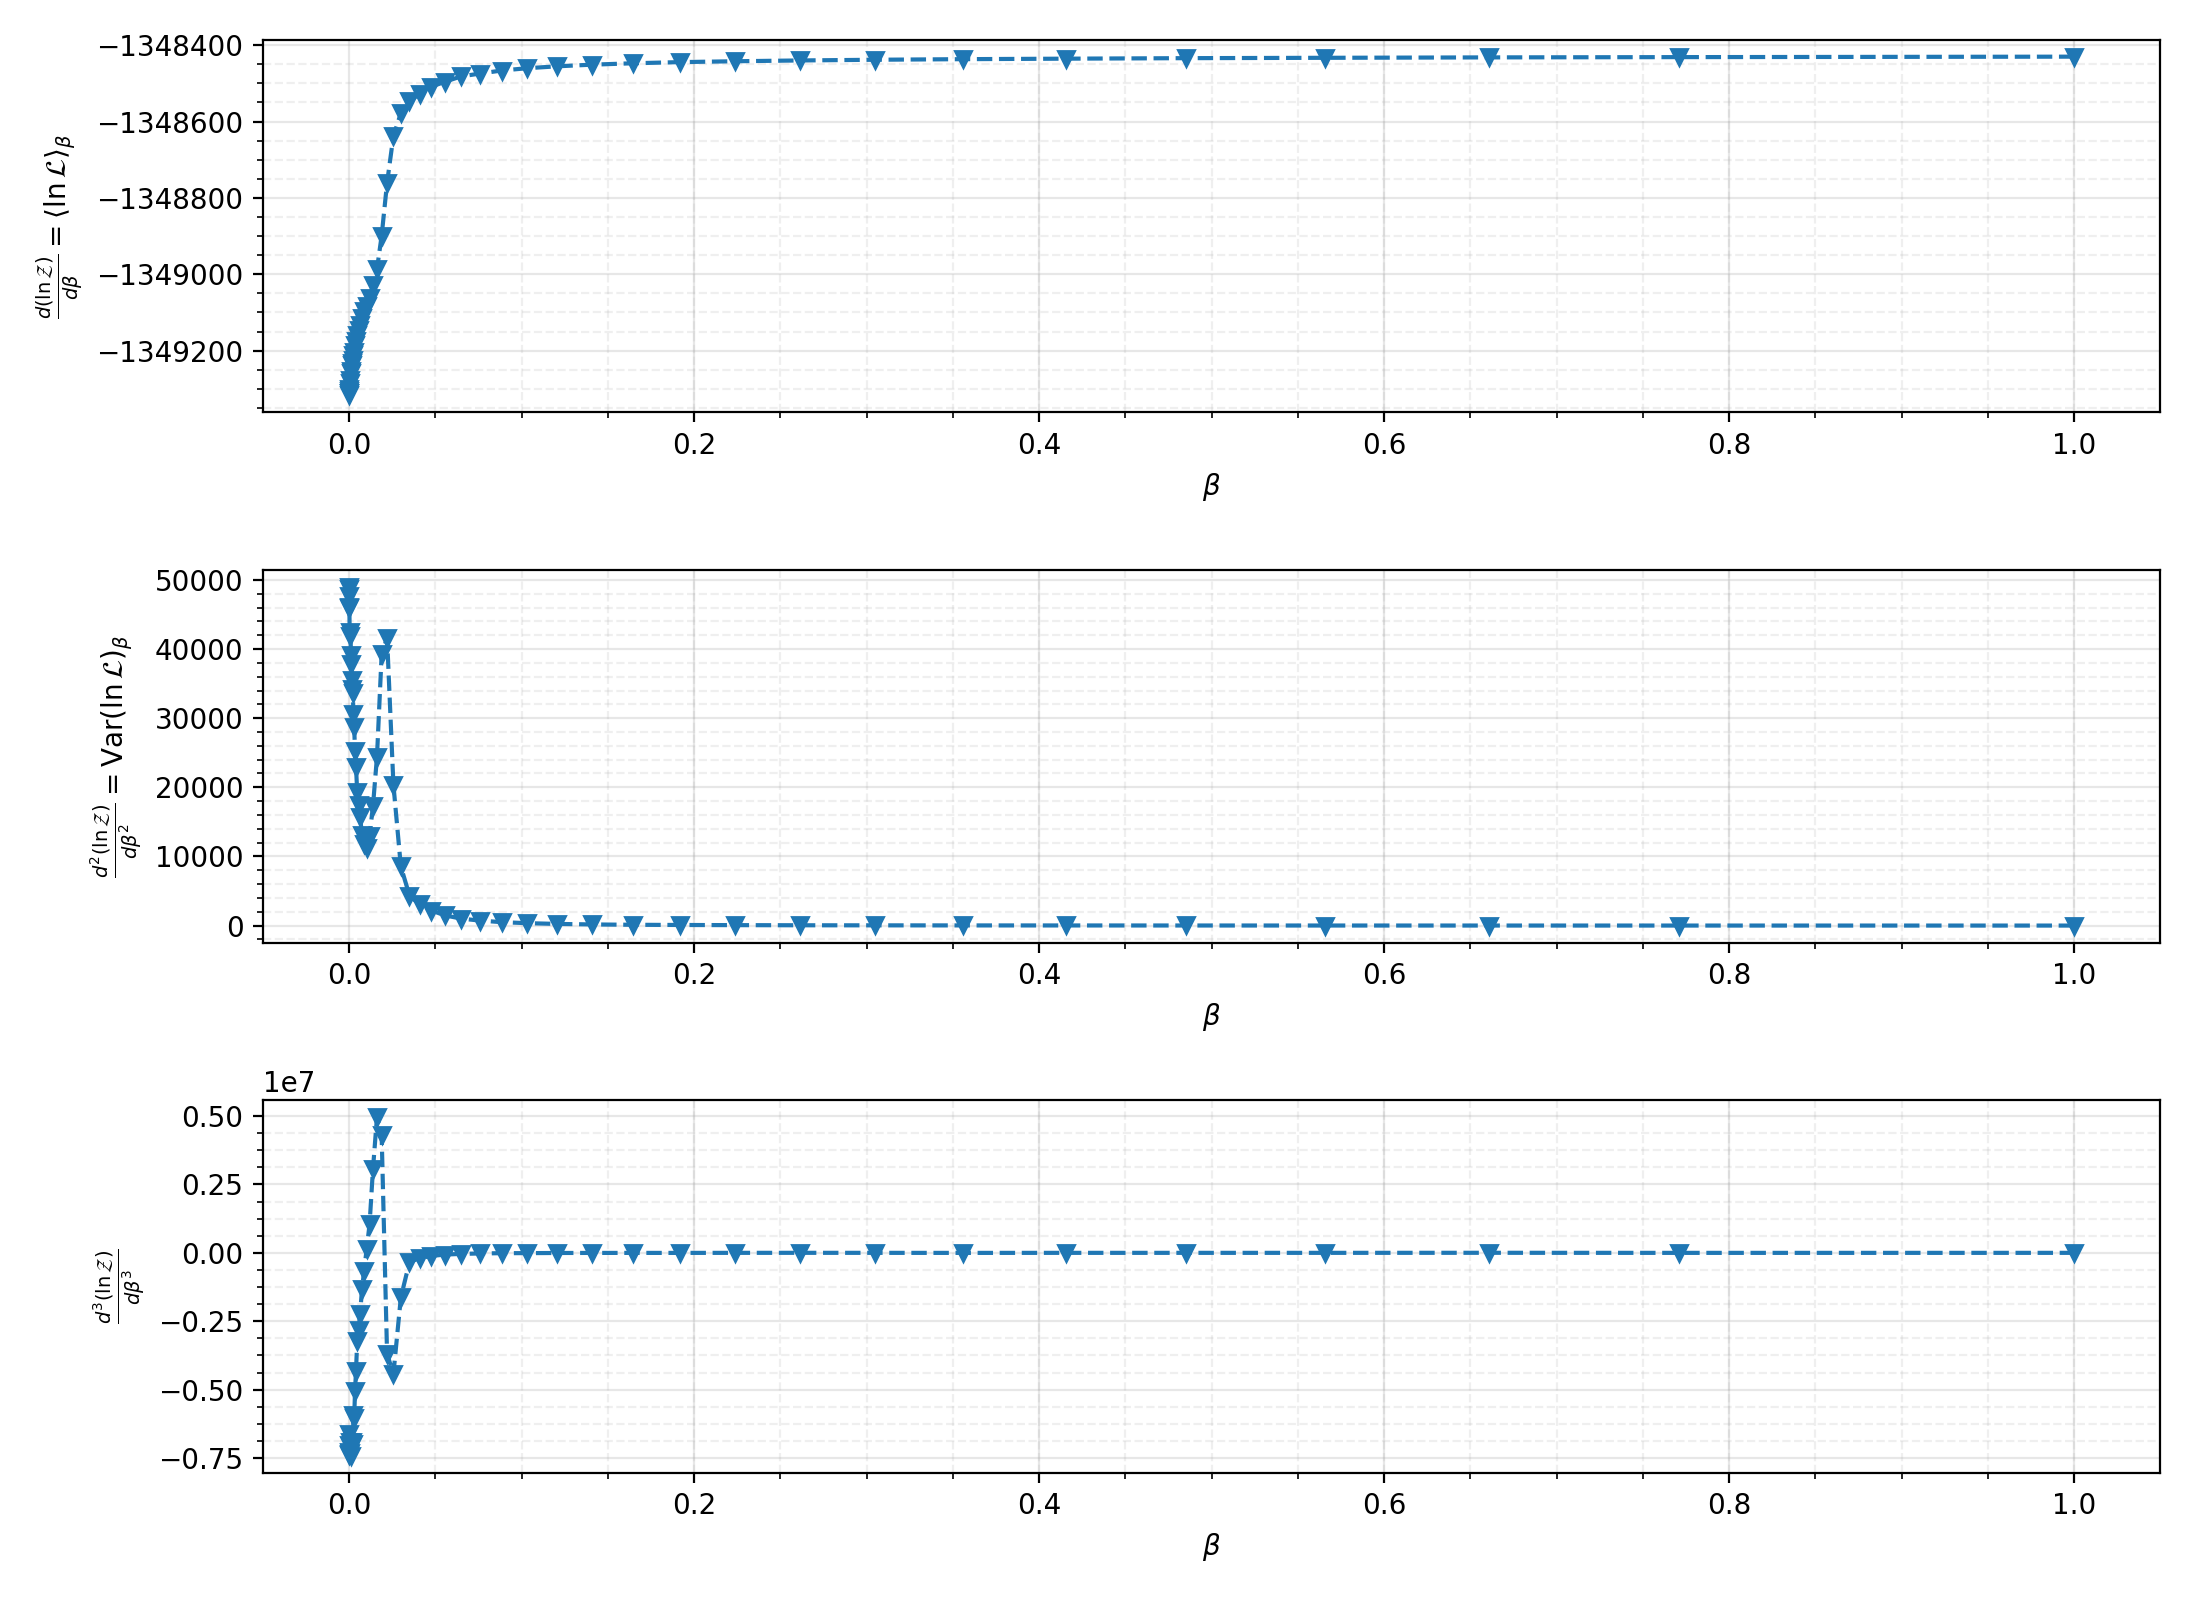
\includegraphics[width=1.0\textwidth]{figs/chapter6/gooseneck_plots_linear.png}
\caption{The subplots of the thermodynamic integrand and subsequent derivatives of the thermodynamic integral. (\textit{Top}) The thermodynamic integrand when compared to the inverse-temperature $\beta$. The curve should be smooth and montonic, however it is very difficult to inspect the integrand on a linear $\beta$ scale. (\textit{Middle}) The second derivative of the logarithm of the evidence is the variance of the power-posterior at an inverse temperature $\beta$. There is some indication that an inflection point happens in the curvature of the integrand at high temperature. (\textit{Bottom}) The third derivative of the logarithm of the evidence is also the third-order cumulant of the power-posterior distributions at an inverse-temperature $\beta$. It is difficult to inspect the behavior of this derivative on the linear $\beta$ scale.}
\label{fig:gooseneck_linear}
\end{figure}

\begin{figure}[th]
\centering
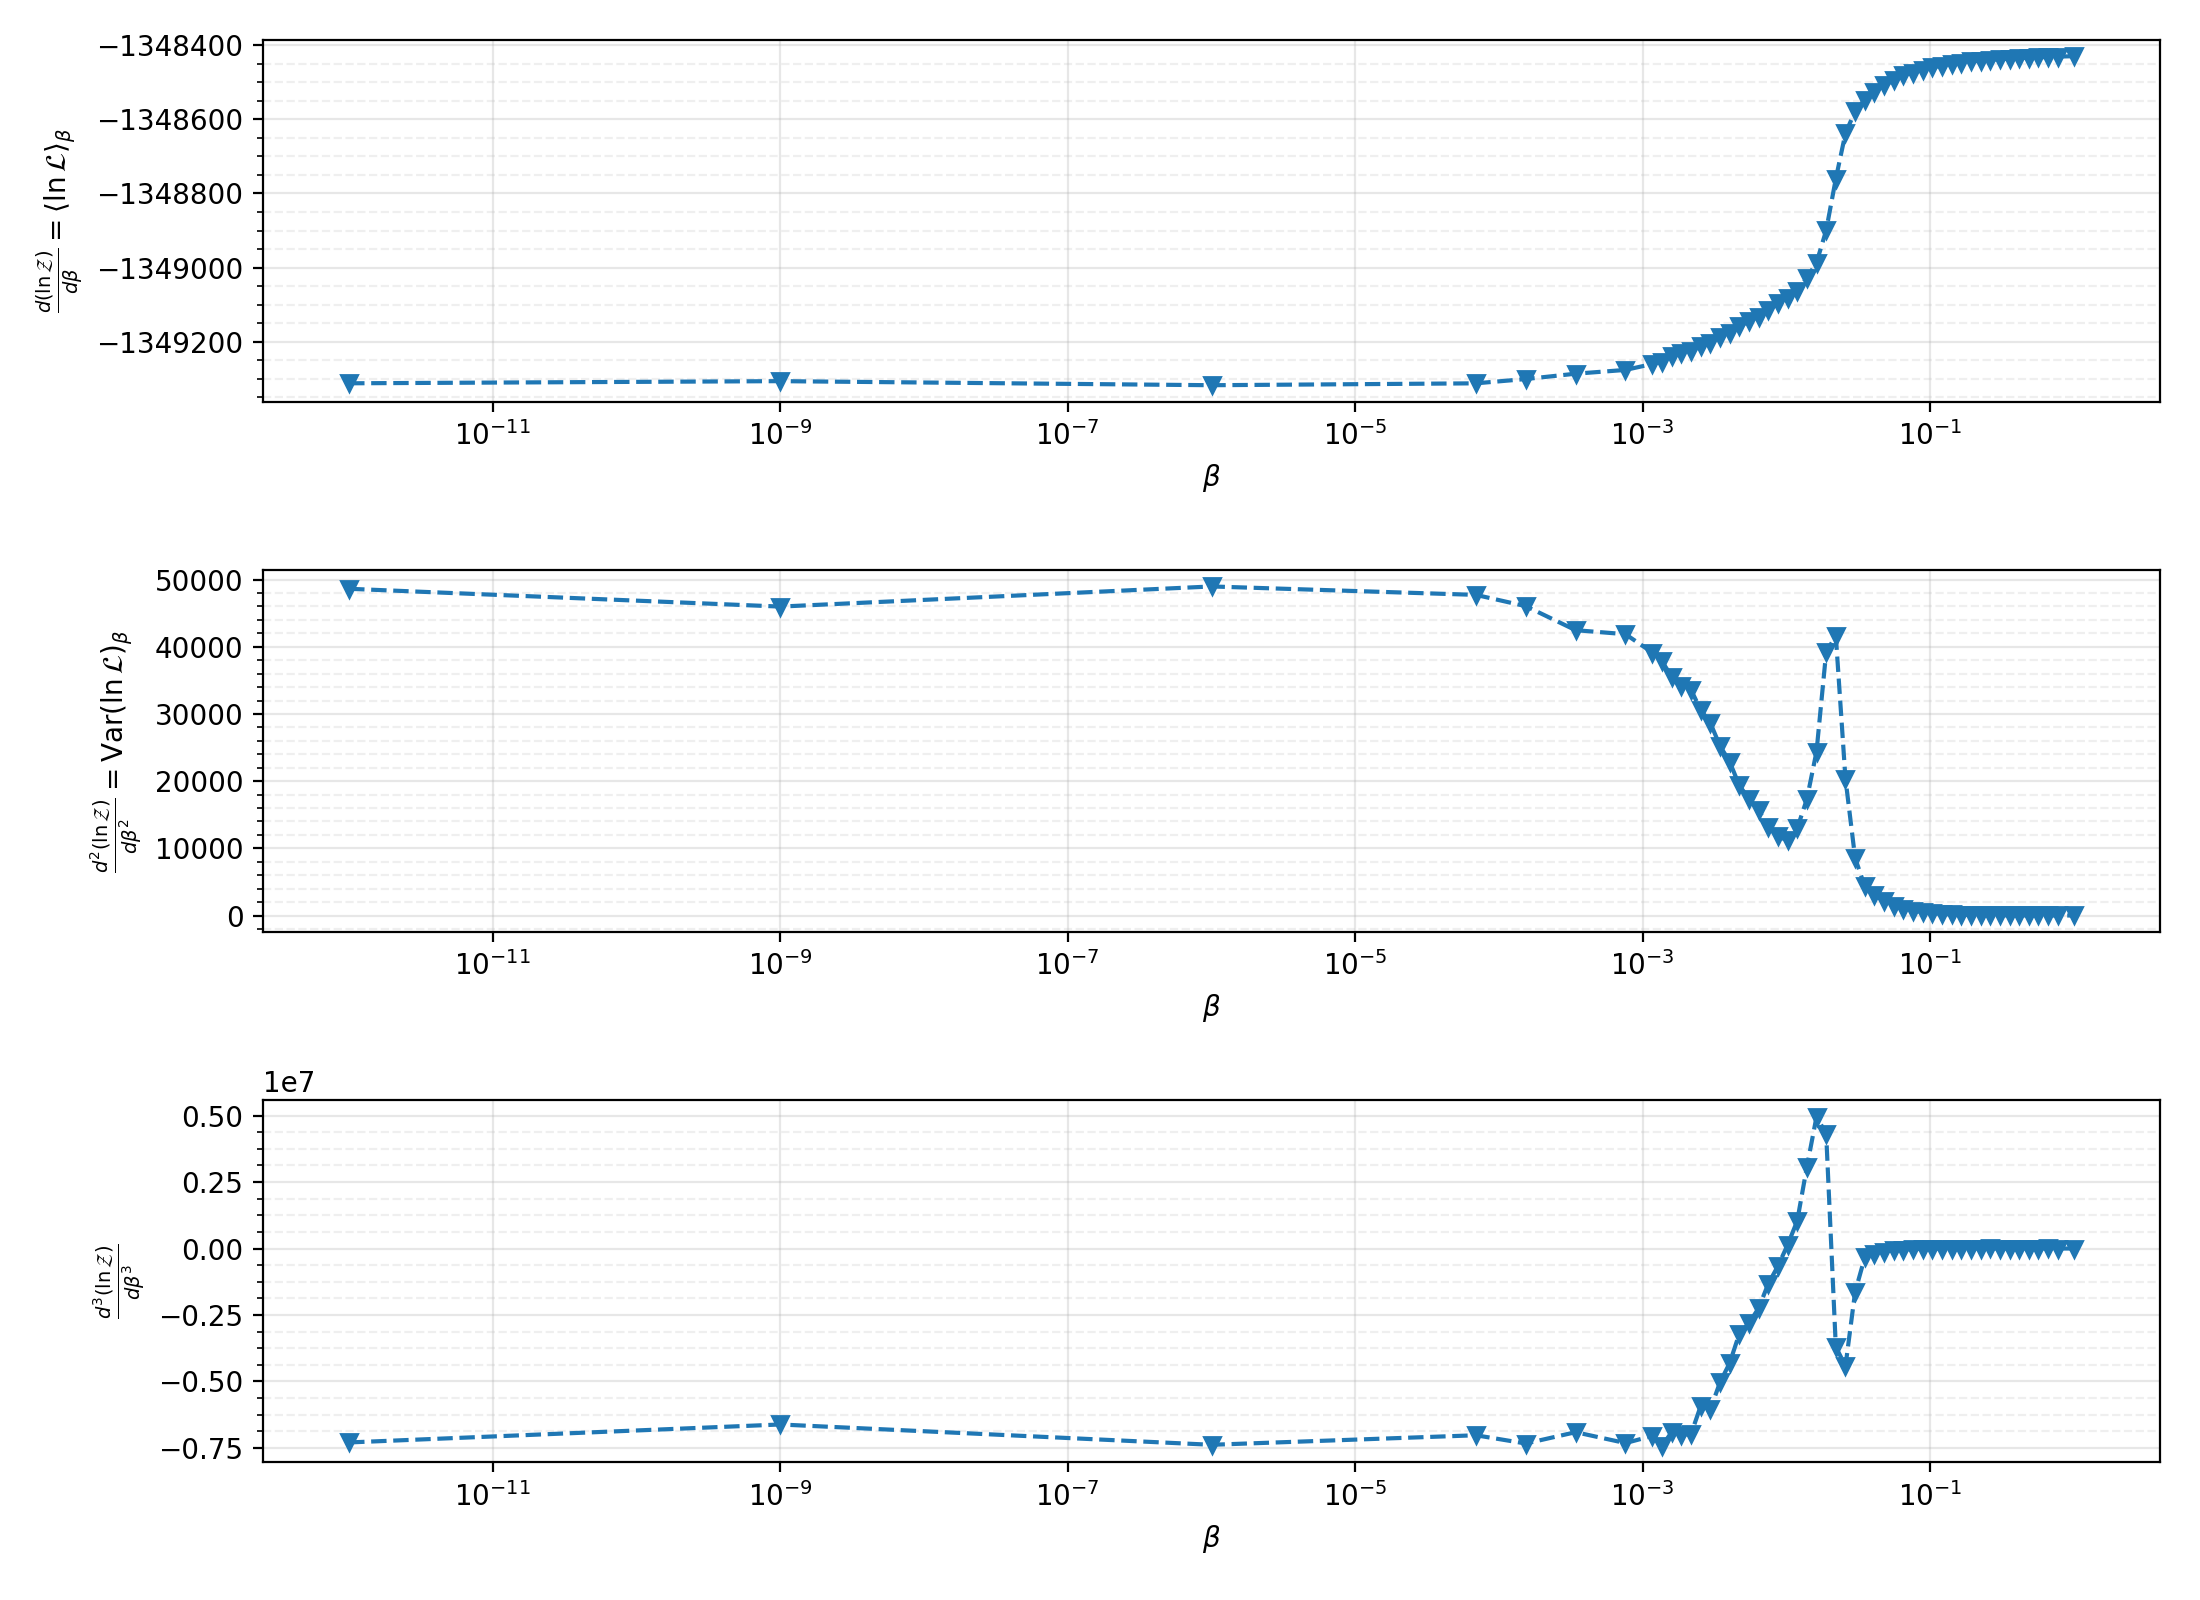
\includegraphics[width=1.0\textwidth]{figs/chapter6/gooseneck_plots_log.png}
\caption{The subplots of the thermodynamic integrand and subsequent derivatives of the thermodynamic integral. (\textit{Top}) The thermodynamic integrand when compared to the inverse-temperature $\beta$. The curve should be smooth and montonic, however there is some indication at $\beta = 10^{-9}$ that this condition is not strictly met in the Markov Chain Monte Carlo simulation. (\textit{Middle}) The second derivative of the logarithm of the evidence is the variance of the power-posterior at an inverse temperature $\beta$. This function should also be smooth however there is some indication that at high temperature that the derivatives are not stable. (\textit{Bottom}) The third derivative of the logarithm of the evidence is also the third-order cumulant of the power-posterior distributions at an inverse-temperature $\beta$. Here we can see that the derivatives are not very sable or smooth. This may motivate moving our analysis to new multi-tempered samplers that are optimized for thermodynamic integration.}
\label{fig:gooseneck_log}
\end{figure}

\subsection{Numerical Quadrature}
The thermodynamic integral in Eq.~(\ref{eq:thermoint}) can be estimated through numerical quadrature rules such as the trapezoidal rule or Simpson's rule. However, a good placement for the inverse-temperatures $\beta$ for accurate thermodynamic integration is not typically uniformly distributed between $0$ and $1$. Therefore it is helpful to consider integration rules that do not depend on equally spaced abscissa ($\beta$ in the context of thermodynamic integration). A polynomial interpolant that does not make use of derivatives of the function or equally spaced abscissa is the Newton's divided difference interpolant, see~\cite{brun1953generalization, selmer1958numerical, abramowitz1965handbook} for examples of how to construct these polynomials. Other interpolants, and thus integration rules, can also be constructed, see ~\cite{abramowitz1965handbook} for examples.

The simplest rule that we consider here is the trapezoidal rule which can be written for thermodynamic integration as:
\begin{equation}
    \widehat{\mathrm{ln} \, \mathcal{Z}}_{\mathrm{Trapz}} = \sum_{i=0}^{N_\beta-1} \frac{1}{2} \left(\beta_{i+1} - \beta_i \right) \left(\langle \mathrm{ln} \, \mathcal{L} \rangle_{\beta_{i+1}} + \langle \mathrm{ln} \, \mathcal{L} \rangle_{\beta_{i}} \right)
\end{equation}
Here $N_\beta$ represents the number of $\beta$ being summed over in the integration estimation. The error corrective term to the trapezoidal rule can be found by integrating the next-to-leading order Taylor polynomial correction~\citep{abramowitz1965handbook}, yielding:
\begin{equation}
    \widehat{\mathrm{ln} \, \mathcal{Z}}_{\mathrm{Trapz \, +}} \approx \widehat{\mathrm{ln} \, \mathcal{Z}}_{\mathrm{Trapz}} + \sum_{i=0}^{N_\beta-1} -\frac{1}{12} \left(\beta_{i+1} - \beta_i \right)^2 \left(f'(\beta_{i+1}) - f'(\beta_{i}) \right).
\end{equation}
Here $f'(\beta_i)$ represents the second derivative of $\mathrm{ln} \, \mathcal{Z}$ with respect to $\beta$. It was found in~\cite{friel2014improving} that this corresponds to the variance of the untempered log likelihood as drawn from the power-posterior at $\beta_i$.

Simpson's rule for unequally spaced abscissa under Newton's divided difference interpolation~\citep{easa1988area} is:
\begin{equation}
    \widehat{\mathrm{ln} \, \mathcal{Z}}_{\mathrm{Simps}} = \sum_{\mathrm{i\, is\, even}, \\ i=0}^{N_\beta-2} \frac{h_i + h_{i+1}}{6} \left [ A \, \langle \mathrm{ln} \, \mathcal{L} \rangle_{\beta_{i}} + B \, \langle \mathrm{ln} \, \mathcal{L} \rangle_{\beta_{i+1}} + C \, \langle \mathrm{ln} \, \mathcal{L} \rangle_{\beta_{i+2}}\right ],
\end{equation}
for the expressions:
\begin{equation}
\begin{array}{lll}
     A &= \frac{(2h_i - h_{i+1})}{h_i} \\ \\ 
     B &= \frac{(h_i+h_{i+1})^2}{h_i h_{i+1}} \\ \\
     C &= \frac{(2h_{i+1} - h_i)}{h_{i+1}}. \\ \\
\end{array}
\end{equation}
Here  $h_i \equiv \beta_{i+1} - \beta_i$, and $h_{i+1} \equiv \beta_{i+2} - \beta_{i+1}$. The error corrective term for Simpson's rule can thus be solved in the same manner as for the trapezoidal rule and we find:
\begin{equation}
    \widehat{\mathrm{ln} \, \mathcal{Z}}_{\mathrm{Simps \, +}} \approx \widehat{\mathrm{ln} \, \mathcal{Z}}_{\mathrm{Simps}} + \sum_{\mathrm{i\, is\, even}, \\ i=0}^{N_\beta-2} \frac{1}{72}\left(\beta_{i+2} - \beta_{i} \right)^2 (\beta_i - 2\beta_{i+1} + \beta_{i+2})\frac{f''(\beta_{i+2}) - f''(\beta_i)}{\beta_{i+2} - \beta_i}.
\end{equation}
Here $f''(\beta_i)$ represents the third derivative of $\mathrm{ln} \, \mathcal{Z}$ with respect to $\beta$, which is in Eq.~\ref{eqn:third_ti_deriv}.

The cubic integration rule for unequally spaced abscissa under Newton's divided difference interpolation can be found in~\cite{brun1953generalization,selmer1958numerical,chambers1989estimating} or can be derived through the tools in~\cite{abramowitz1965handbook}. We present the form given in~\cite{chambers1989estimating}:
\begin{equation}
    \widehat{\mathrm{ln} \, \mathcal{Z}}_{\mathrm{cubic}} = \sum_{\mathrm{i\, is\, a \, multiple \, of \, 3}, \\ i=0}^{N_\beta-3} \frac{h_i + h_{i+1} + h_{i+2}}{12} \left [A \, \langle \mathrm{ln} \, \mathcal{L} \rangle_{\beta_{i}} + B \, \langle \mathrm{ln} \, \mathcal{L} \rangle_{\beta_{i+1}} + C \, \langle \mathrm{ln} \, \mathcal{L} \rangle_{\beta_{i+2}} + D \, \langle \mathrm{ln} \, \mathcal{L} \rangle_{\beta_{i+3}}\right ],
\end{equation}
for expressions:
\begin{equation}
\begin{array}{llll}
     A &= \frac{3h_i^2 -h_{i+1}^2 +h_{i+2}^2 +2 h_i h_{i+1} - 2h_i h_{i+2}}{h_i (h_i + h_{i+1})} \\ \\
     B &= \frac{(h_i + h_{i+1} + h_{i+2})^2 (h_i + h_{i+1} - h_{i+2})}{h_{i} h_{i+1} (h_{i+1} h_{i+2})} \\ \\
     C &= \frac{(h_i + h_{i+1} + h_{i+2})^2 (h_{i+1} + h_{i+2} - h_i)}{h_{i+1} h_{i+2} (h_i + h_{i+1})} \\ \\
     D &= \frac{h_i^2 - h_{i+1}^2 +3 h_{i+2}^2 - 2h_i h_{i+2} + 2 h_{i+1} h_{i+2}}{h_{i+2}(h_{i+1} + h_{i+2})}.\\ \\
\end{array}
\end{equation}
Here we have defined $h_i \equiv \beta_{i+1} - \beta_{i}$, $h_{i+1} \equiv \beta_{i+2} - \beta_{i+1}$, and $h_{i+2} \equiv \beta_{i+3} - \beta_{i+2}$.

We exercise caution in describing the thermodynamic integral through a higher order polynomial quadrature rule as the integrand may not be well interpolated by higher order polynomials. Thus there may be very little incentive for going to higher order polynomial rules as improved accuracy is not always guaranteed by going to higher order polynomial integration rules~\citep{epperson1987runge}. Without prior information on the true logarithm of the evidence we recommend that the available quadrature rules be checked to ensure consistent estimates.

Future studies may make use of Taylor series polynomials for unequally spaced abscissa, ratios of Taylor series polynomials through the Pad$\textrm{\'e}$ approximant for improved accuracy~\citep{press1992pade}, or other interpolant functions. Improvement in numerical integration for thermodynamic integration may also be improved by focusing on increasing the number of inverse-temperatures $\beta$ and/or by improved placement of $\beta$.

\subsection{Monte Carlo Error Estimation}
Here we follow the discussion from \cite{annis2019thermodynamic} who provide a heuristic for estimating the Monte Carlo error to estimating the thermodynamic integral as first given in \cite{friel2008marginal}. A variance of the thermodynamic integral estimator, $\widehat{\mathrm{ln} \, \mathcal{Z}}$, from Monte Carlo error can be found in two steps. First, calculate the thermodynamic integral for each sample of untempered log likelihoods drawn from the power-posterior at $\beta$. For $N$ samples drawn from each power-posterior this generates $N$ thermodynamic integral values. The integration should be done relative to the numerical quadrature technique that one is trying to estimate the Monte-Carlo error for. This represents the sample variance of the thermodynamic integration. The variance of the mean value of the logarithm of the evidence can be calculated via:
\begin{equation}
    \sigma^2_{\mathrm{MC}} = \frac{1}{N} \sigma^2_{\mathrm{sample}}.
\end{equation}
Here, $\sigma^2_{\mathrm{MC}}$ represents the Monte-Carlo variance for the thermodynamic integration estimator while $\sigma^2_{\mathrm{sample}}$ is the sample variance and $N$ represents the number of available samples. See Fig.~\ref{fig:ti_monte_carlo_error} for a visualization of this procedure.

\begin{figure}[th]
\centering
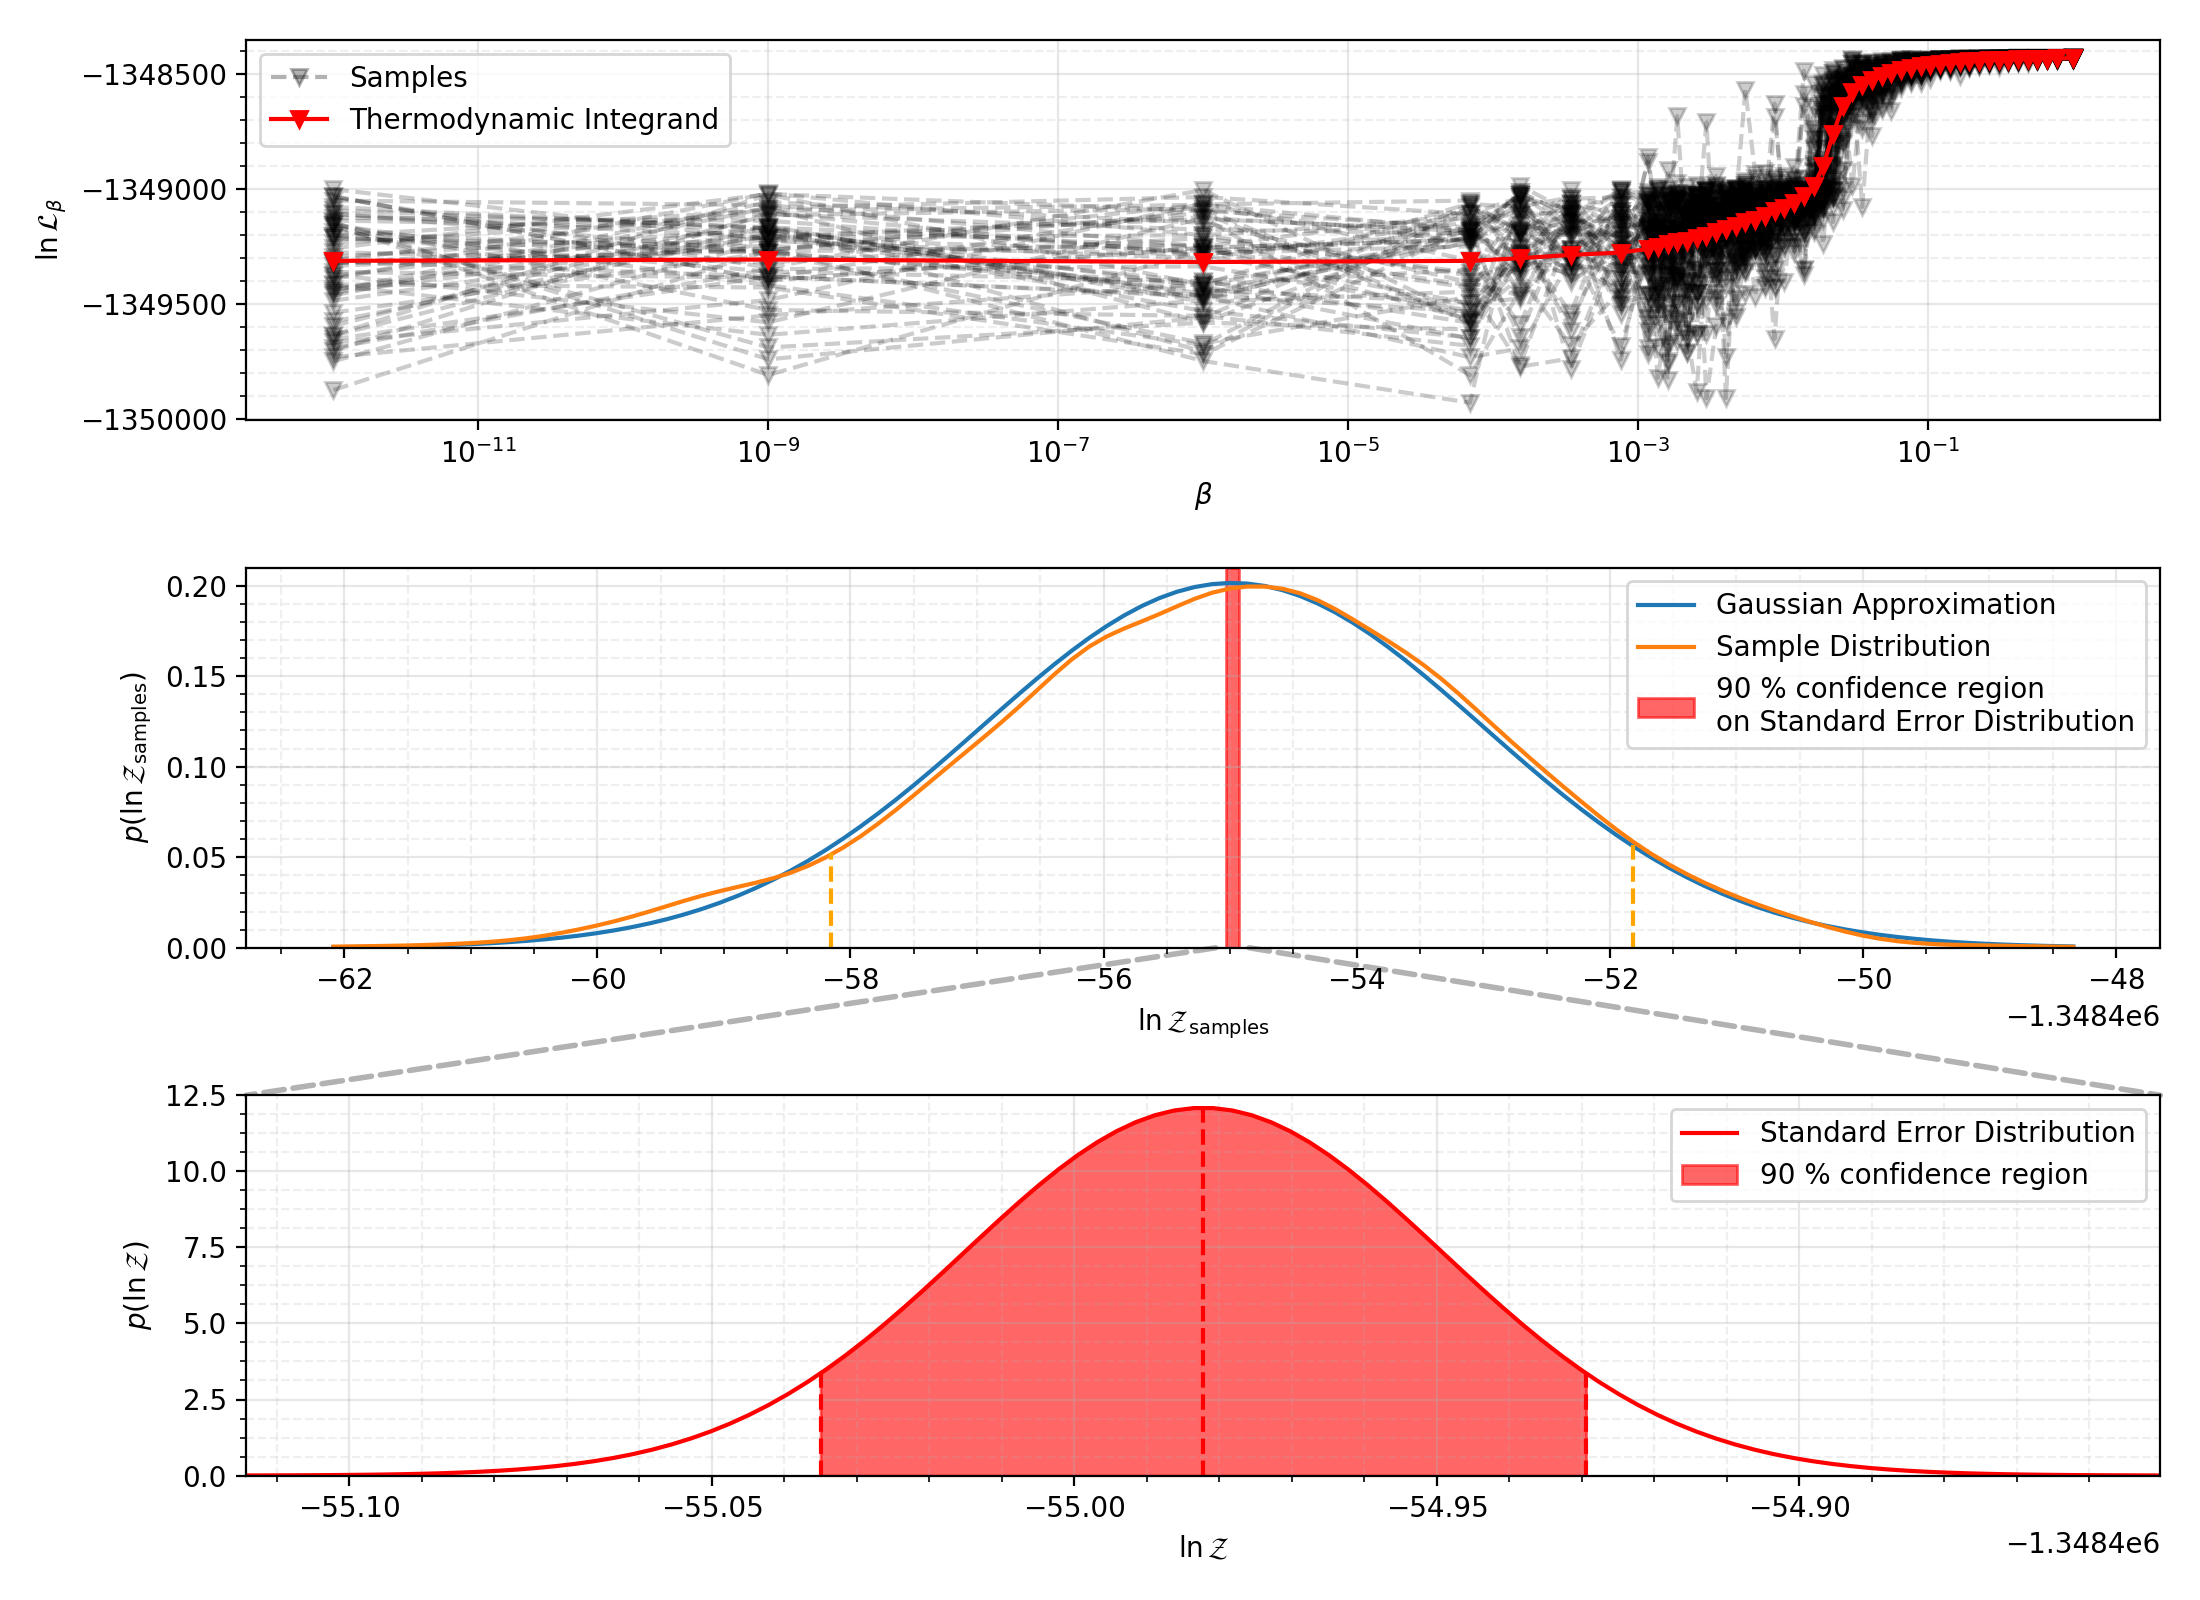
\includegraphics[width=1.0\textwidth]{figs/chapter6/ti_monte_carlo_error.png}
\caption{The first subplot denotes the untempered log-likelihood samples when drawn from the power-posteriors at $\beta$. The expectation value of the untempered log-likelihood when drawn from these power-posteriors is the thermodynamic integrand and is plotted in red. The thermodynamic integral over all geometric paths given from the samples is drawn in the second subplot. The sample-log-integral distribution is approximately a Gaussian distribution. The standard error of the mean value of the log evidence is given by the sample standard deviation divided by the square root of the number of samples. The $90 \%$ confidence interval on the sample distribution in the log-evidence is drawn in dashed orange lines. The $90\%$ confidence region from this standard error is shaded in red. The final subplot is a zoom-in on this $90 \%$ confidence region showing the error estimate on the thermodynamic integral due to Monte Carlo sampling.}
\label{fig:ti_monte_carlo_error}
\end{figure}

Repeated runs where the random seed for the MCMC analysis was changed has shown that the variance estimate from presented in~\cite{annis2019thermodynamic} is a plausible confidence interval estimate for Monte Carlo error.

\subsection{Convergence Error Estimation}
The procedure of estimating the marginal likelihood from power-posterior simulation requires that the power-posteriors all converge to the proper distribution. The simplest approach is to inspect the thermodynamic integrand over the course of the MCMC analysis. It would also require that all of the sequential cumulants of the power-posterior also stabilize, although this is much more difficult to track in practice. In the limit that the MCMC analysis has converged, all of the power-posterior distributions will be stationary with respect to the MCMC progress. To investigate the convergence of the evidence over the course of the MCMC analysis we must be sure to draw independent and identically distributed samples of the chains of the MCMC analysis~\cite{annis2019thermodynamic}.

Gathering independent and identically distributed samples can be done by calculating the autocorrelation length of the MCMC chains at a particular temperature. In practice, \pycbc{}\ Inference calculates the autocorrelation length of all of the temperature chains and uses the largest autocorrelation length as the autocorrelation length for all temperatures~\cite{biwer2019pycbc}. This is a safe and conservative practice for ensuring that samples drawn from the Markov Chain Monte Carlo simulation are not correlated. Thus, to track the thermodynamic integrand at various iterations in the MCMC simulation we divide the MCMC analysis into $12$ equally spaced partitions based on the number of MCMC iterations that the analysis has undergone. In practice any number of partitions will do, but it is computationally intensive to sample more partitions. The partitions do not need to be equally spaced in MCMC iterations but we find equally spaced partitions to be useful for visualization of the progression of the thermodynamic integrand. Using this number of partitions, each partition is segmented in half, where the first half is discarded as burn-in samples, and the autocorrelation length is calculated from the remaining samples. Then independent samples are drawn from this segment spaced out by the calculated autocorrelation length. This is the generic procedure of the $\mathrm{n_{acl}}$ algorithm implemented in \pycbc{}\ for drawing independent samples from the Markov chains~\cite{biwer2019pycbc}. The partitioning procedure is shown in Fig.~\ref{fig:nacl_segments}.

Having drawn independent samples from $12$ segments of the MCMC analysis we can visually inspect the stability of the thermodynamic integrand at $12$ iterations in the MCMC analysis. We can also inspect the convergence of the thermodynamic integral. When the logarithm of the evidence has converged to $\mathcal{O}(10^{-2}$ accuracy, we usually consider the power-posteriors to have converged to their final stationary distribution. Figure~\ref{fig:integrand_convergence} shows the progression of the convergence of the thermodynamic integrand as a function of the MCMC iteration. Figure~\ref{fig:integral_convergence} shows the convergence rate of the thermodynamic integral as a function of the MCMC iteration for a variety of integration techniques.

\begin{figure}[th]
\centering
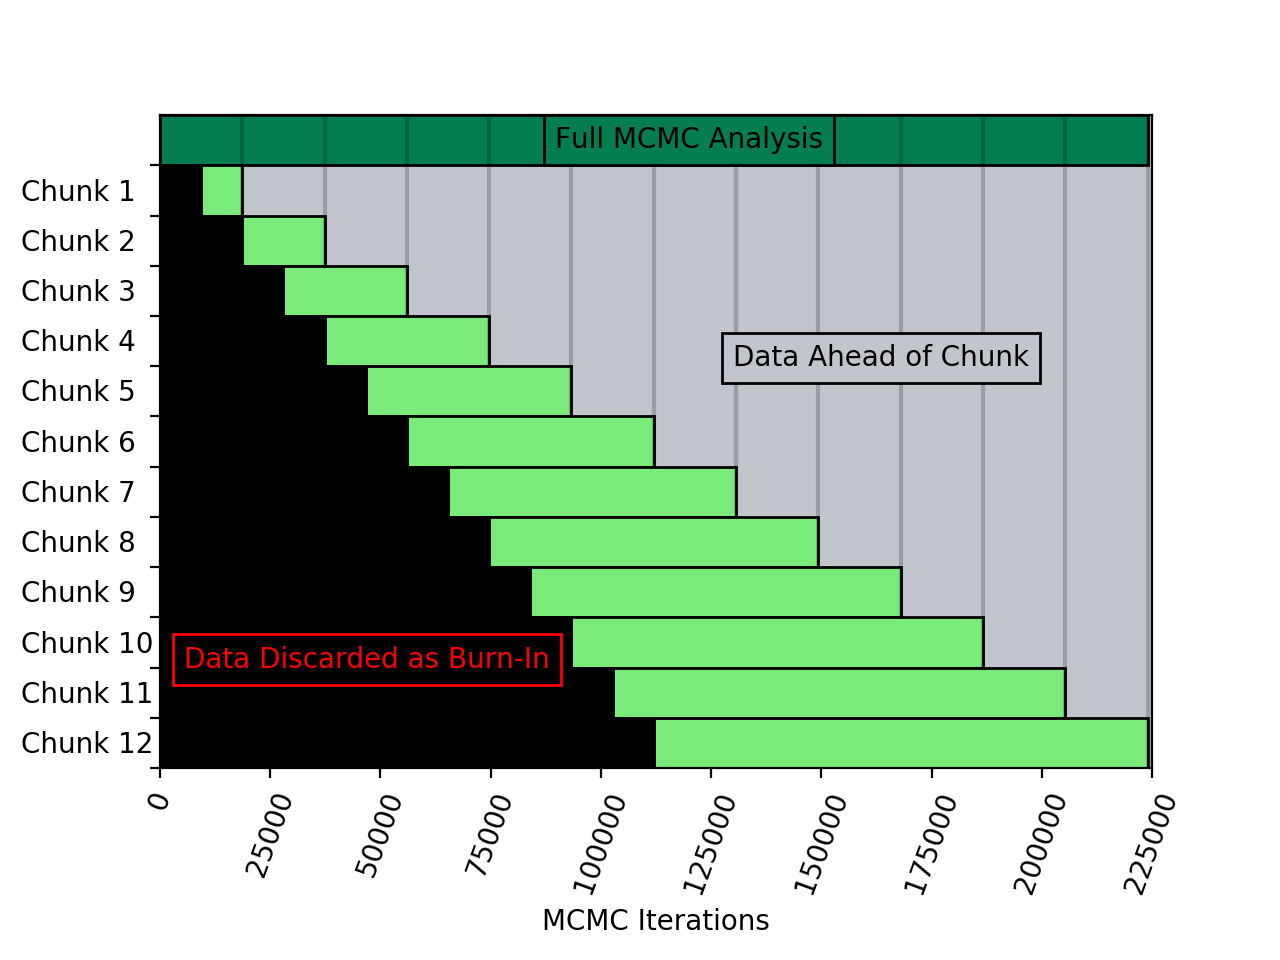
\includegraphics[width=1.0\columnwidth]{figs/chapter6/convergence_segmentation_lvc_sim.png}
\caption{The partitioning of the MCMC analysis to check on the convergence of the thermodynamic integrand and the thermodynamic integration. The dark-green bar at the top represents all of the samples collected by the MCMC analysis. This segment is divided into 12 segments represented by the light gray lines. The light-green segments represent chunks that independent samples can be drawn from. The dark region represents samples discarded as burn-in samples for the MCMC. The dark grey region represents data that is ahead of the chunk and thus not used in drawing independent samples for that chunk. Chunk $12$ produces the identical samples as drawing independent samples according to the $\mathrm{n_{acl}}$ algorithm from PyCBC at the end of the analysis.}
\label{fig:nacl_segments}
\end{figure}

\begin{figure}[th]
\centering
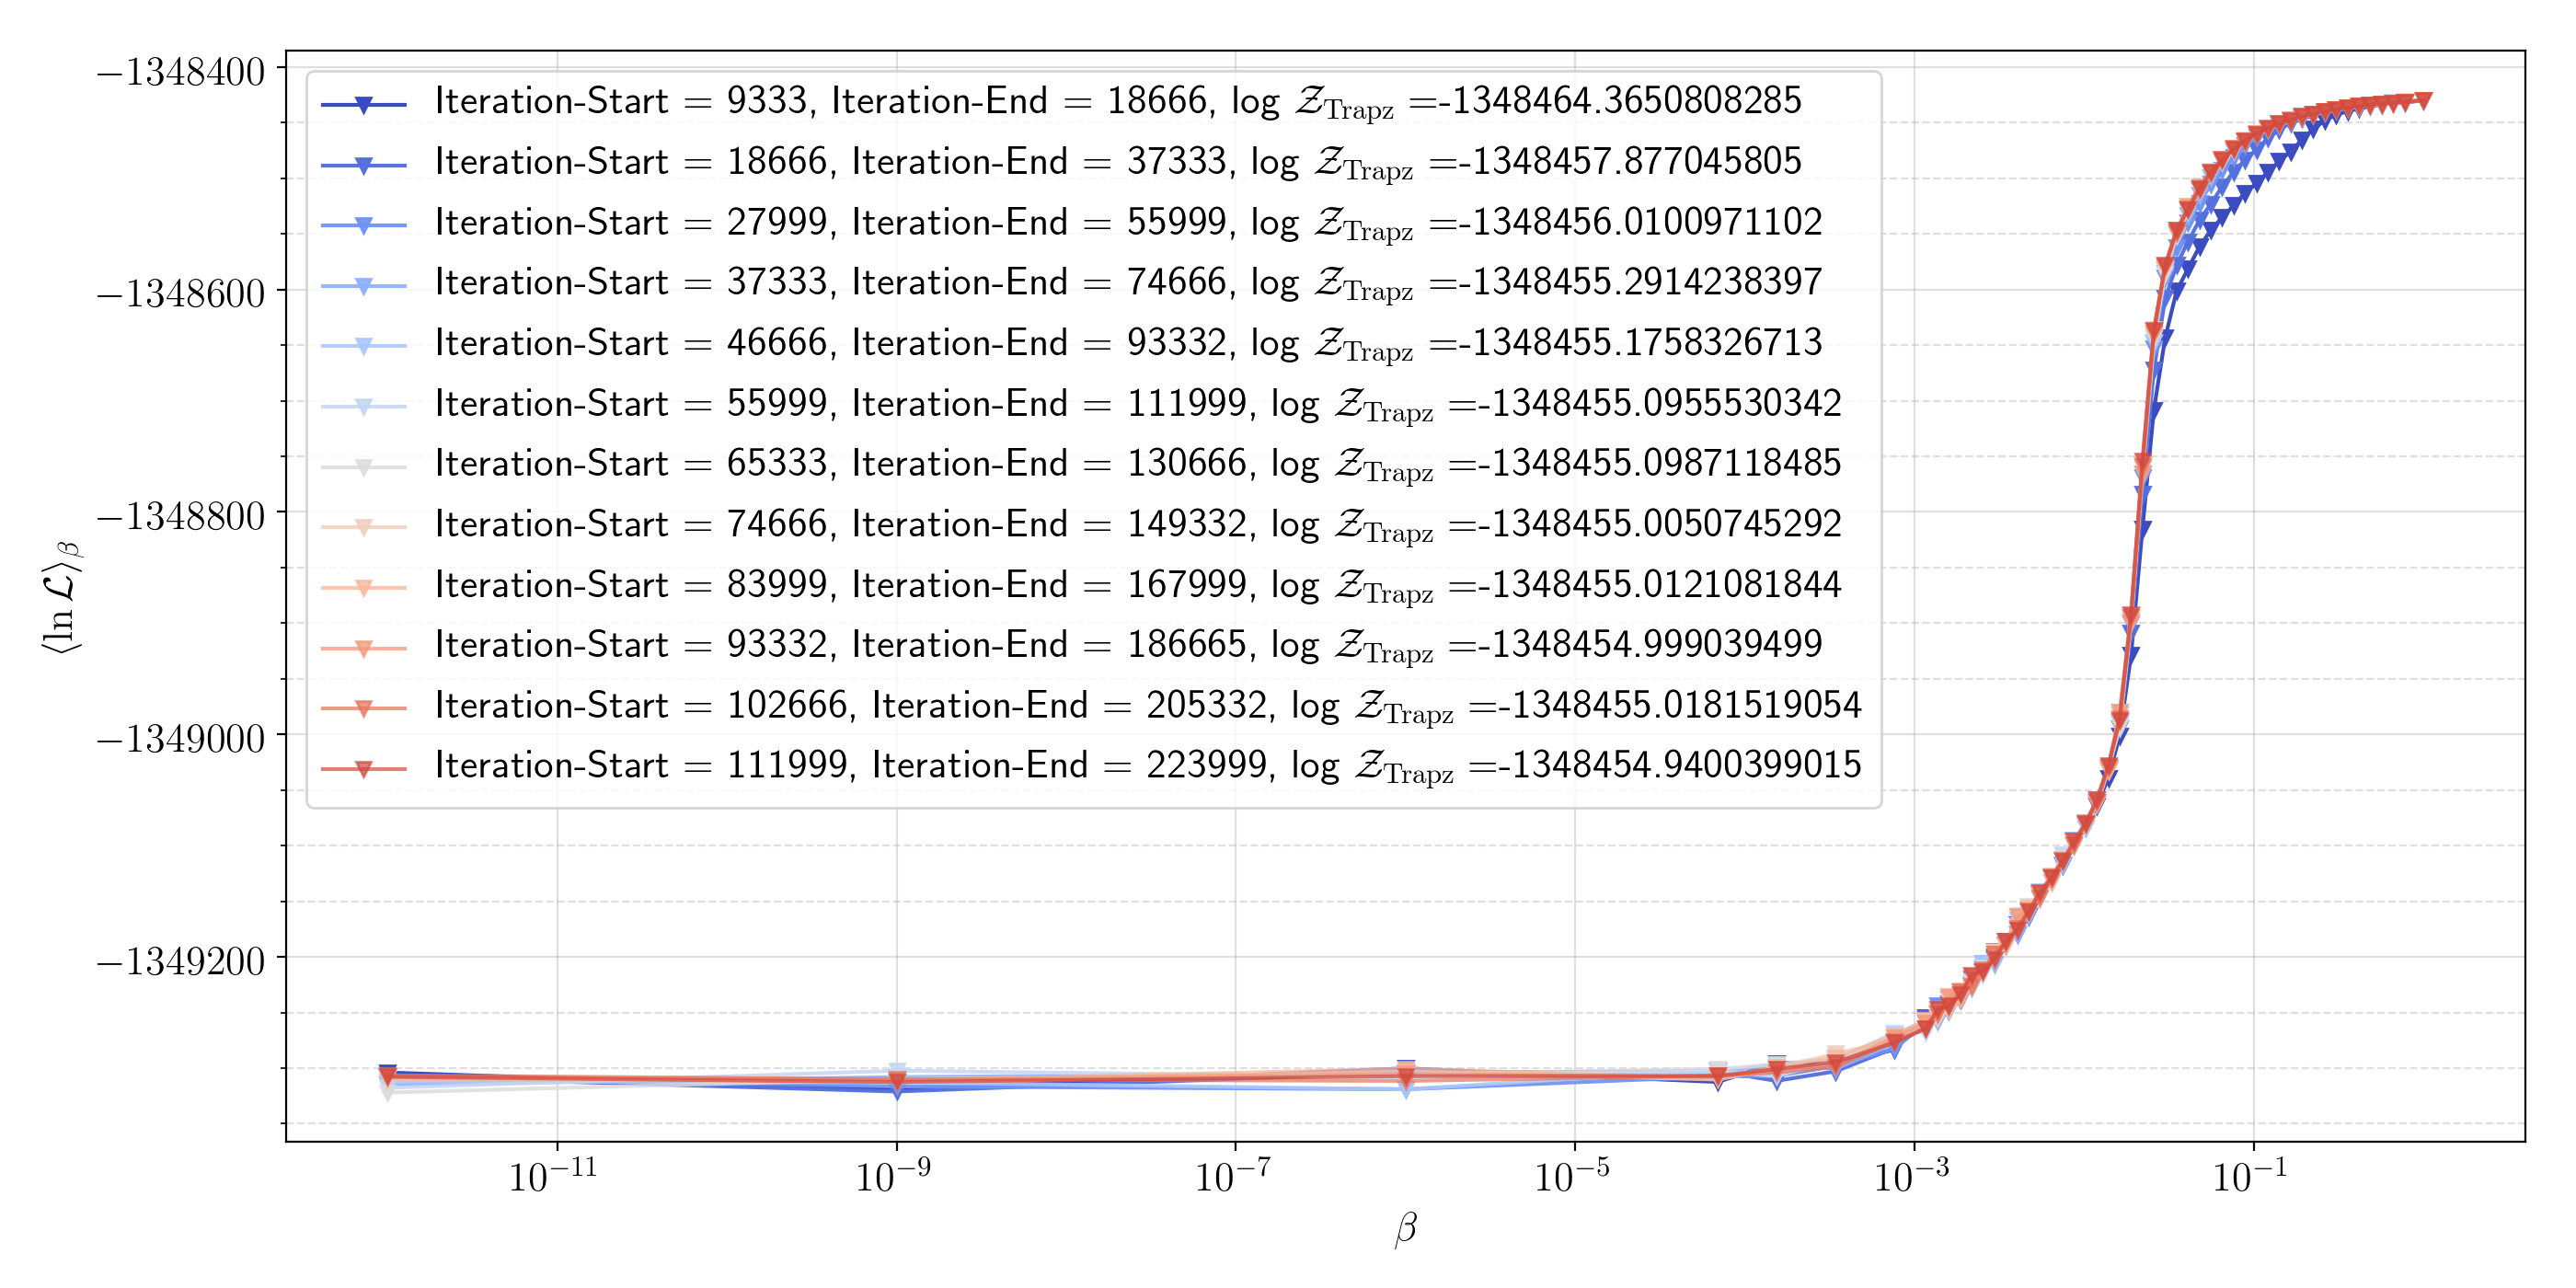
\includegraphics[width=1.0\columnwidth]{figs/chapter6/lsc_sim_integrand_progress.png}
\caption{The convergence of the thermodynamic integrand for a gravitational wave analysis using $51$ temperatures. This analysis neglected $\beta$ = $0$, but is otherwise an acceptable representation of the thermodynamic integrand. The Iteration-Start denotes the point is taken from a segment beginning with that MCMC iteration and ending with the MCMC iteration denoted as Iteration-End. These iterations correspond to the segments found in Fig.~\ref{fig:nacl_segments}. The logarithm of the evidence is shown also in the figure caption, and as the MCMC analysis progresses the integral converges to a set value. The thermodynamic integrand can be visually seen to converge to a S-like curve but the shape and curvature are unique to hypotheses and choice of data. Early in the MCMC analysis the thermodynamic integrand can be mishaped as the power-posteriors have not all converged. Experience has told us tha the power-posteriors that take the longest to converge tend to be in the region where the average log likelihood changes rapidly. Here this is in the region between $\beta$ $\in$ ($10^{-2} - 1$).}
\label{fig:integrand_convergence}
\end{figure}

\begin{figure}[th]
\centering
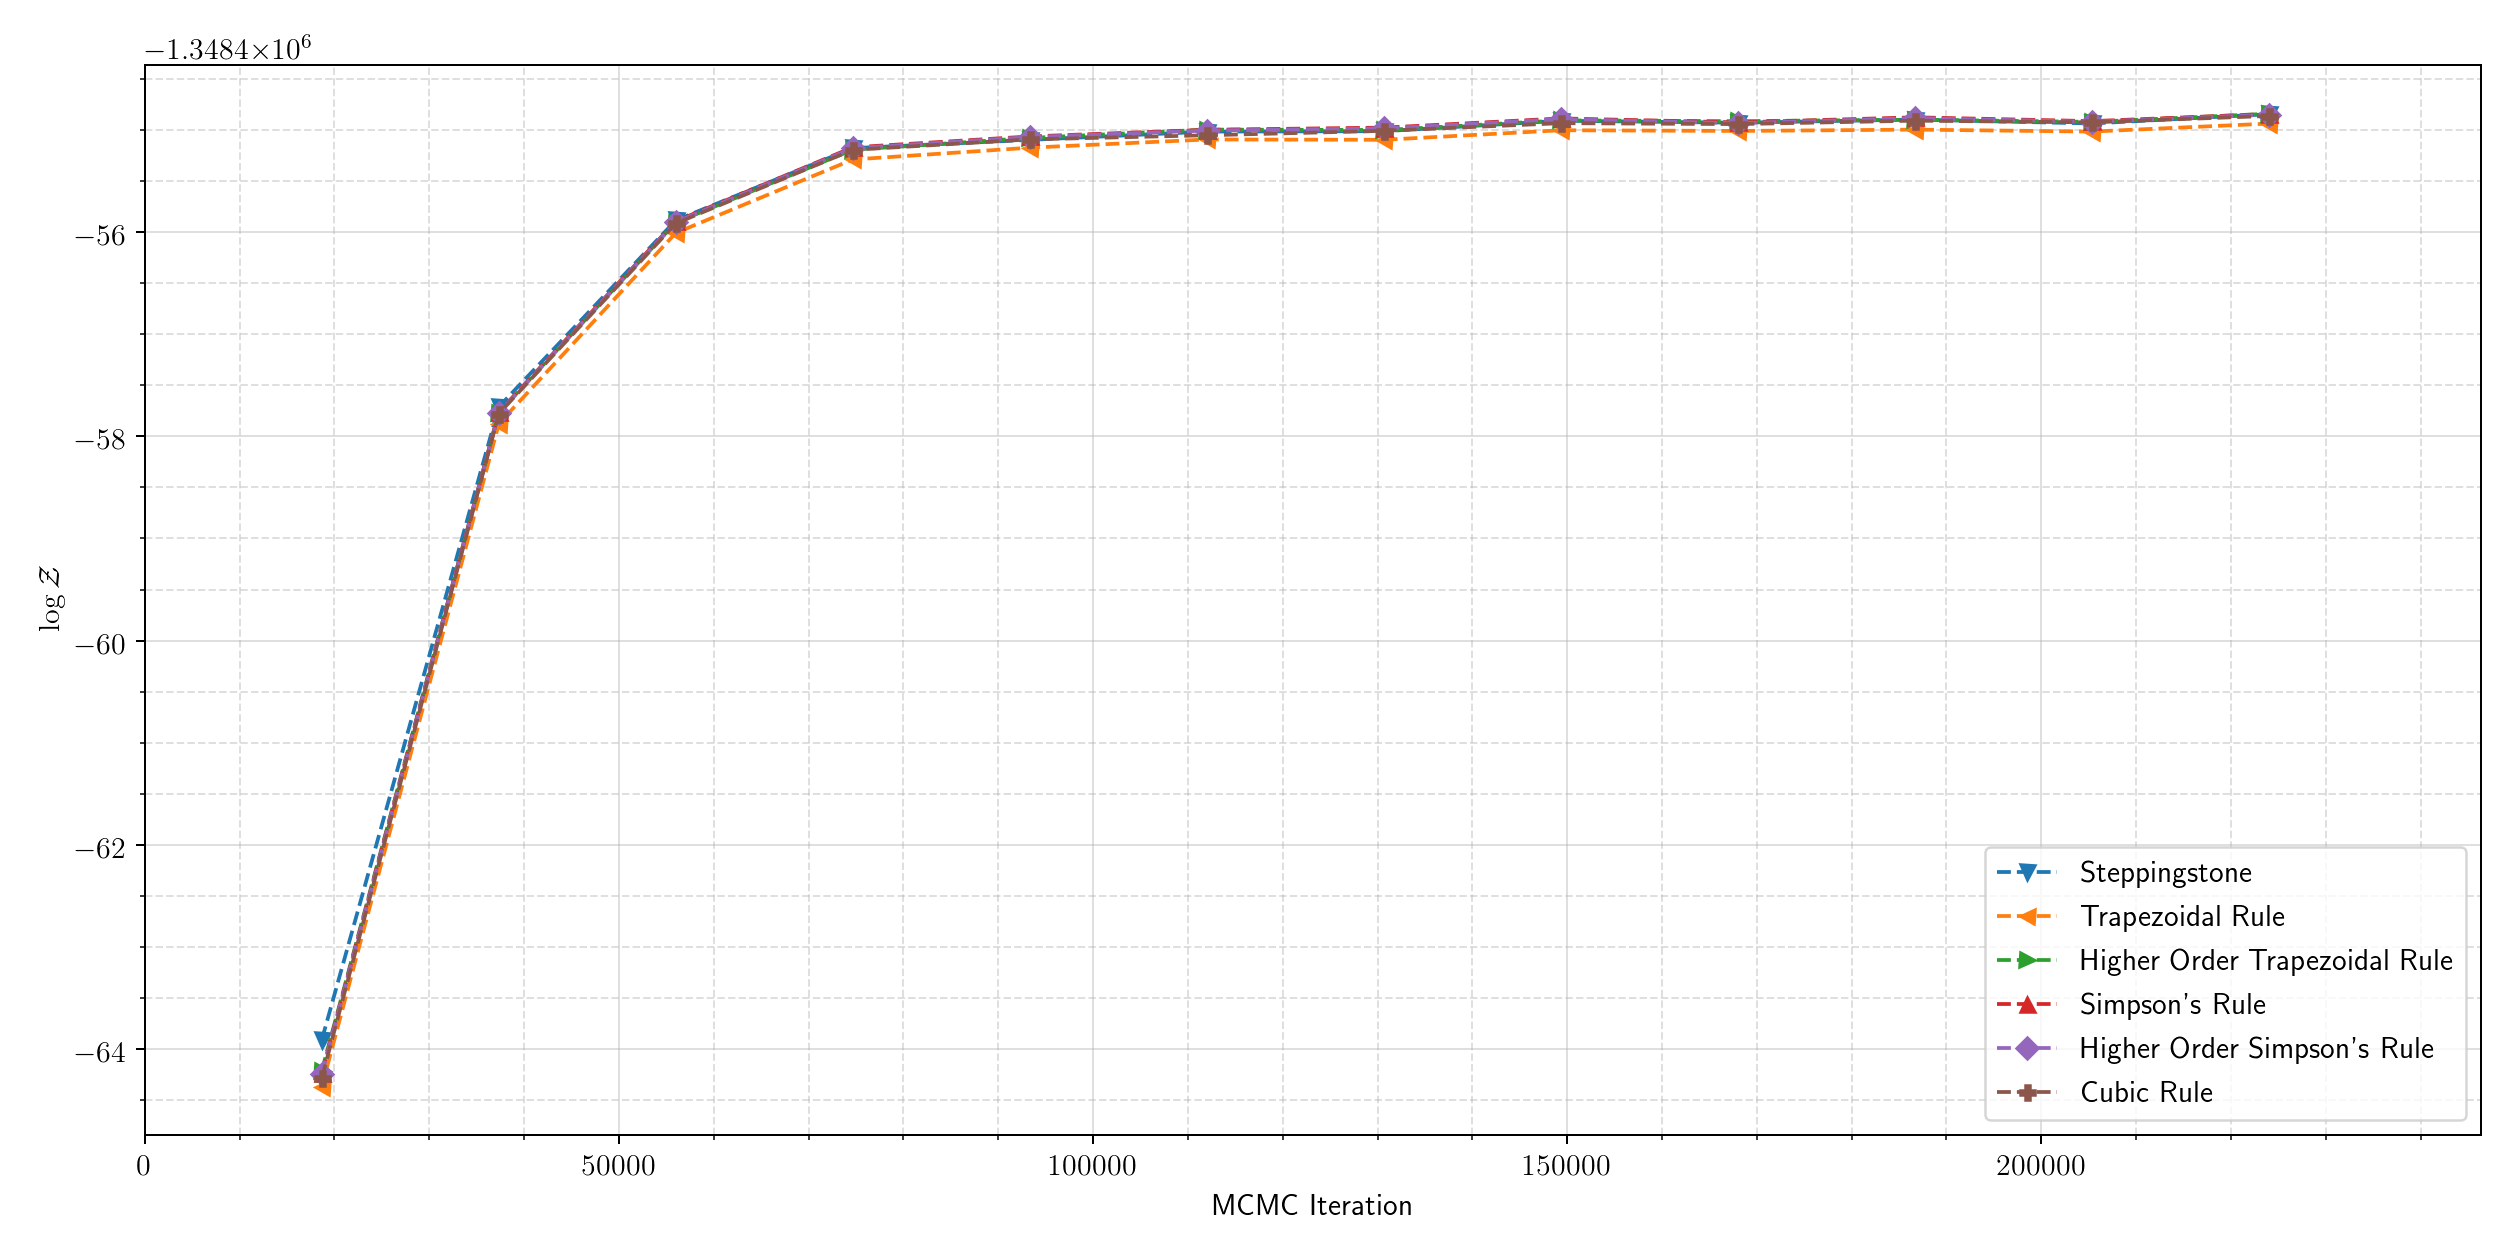
\includegraphics[width=1.0\columnwidth]{figs/chapter6/lvc_sim_evidence_convergence.png}
\caption{The convergence of the thermodynamic integral for a gravitational wave analysis using $51$ temperatures as a function of the MCMC iteration. These choice of points of iterations correspond to the segments found in Fig.~\ref{fig:nacl_segments}. As the analysis progresses the logarithm of the evidence from all quadrature methods tend towards a fixed value.}
\label{fig:integral_convergence}
\end{figure}

Finally, the absolute value of the difference between the last two thermodynamic integration estimates from this partitioning are then used as the standard deviation of the error for the log evidence due to convergence error, $\sigma_{\mathrm{convergence}}$:
\begin{equation}
    \sigma_{\mathrm{convergence}} \sim  \, \mid \mathrm{ln} \, \mathcal{Z}_{\mathrm{partition \,} N} - \mathrm{ln} \, \mathcal{Z}_{\mathrm{partition \,} N-1} \mid
\end{equation}
This provides a rough estimate for estimating the consequences of potentially terminating the MCMC analysis too early.

During the development of this technique a similar technique based on a moving-block bootstrap method was developed in~\cite{Russel:2018pqv} for error analysis of the logarithm of the evidence from the thermodynamic integration method. We have not investigated this technique thoroughly to compare its performance with our own method.

\subsection{Temperature Placement Bias}
The placement of inverse-temperatures $\beta$ also affects the results of the numerical integration for the evidence\citep{lartillot2006computing, xie2010improving}. Research into the proper placement of $\beta$ is ongoing in the field of Statistics~\citep{calderhead2009estimating, annis2019thermodynamic}. It is suggested in~\cite{liu2016evaluating, de2013comparison} that inverse-temperatures should be placed where the thermodynamic integrand changed rapidly or by inspecting the derivatives of the thermodynamic integrand. It is recommended ~\cite{annis2019thermodynamic} that more than $40$ temperatures be used, and we have found $>50$ inverse-temperatures to be a good rule of thumb in the context of gravitational wave data analysis. 

One method for improved temperature placement would be to use the intersection of the slopes of the thermodynamic integrand from two adjacent power-posteriors as a new position for additional temperatures as suggested in~\cite{friel2014improving}. Or it may also be possible to use Bayesian inference and Bayesian quadrature~\cite{diaconis1988bayesian} to improve temperature placement, see ~\cite{briol2015probabilistic} for an application of this procedure with respect to thermodynamic integration.

\section{The Steppingstone Method for Estimating the Bayesian Evidence}
The steppingstone method is very similar in many respects to thermodynamic integration in that it requires multiple inverse-temperatures between $0$ and $1$ to calculate. The steppingstone method uses importance sampling between adjacent temperatures to estimate the contribution to the marginal likelihood $\mathcal{Z}$ at each interval $\beta_{i-1}$-$\beta_i$. Before we present the derivation of the steppingstone method we provide a brief, but useful derivation of another often used identity, called the harmonic mean estimator for the evidence. For the following section we suppress use of $\vec{\theta}$ and $\mathbf{d}$.

For the derivation of the harmonic mean estimator we follow a simplified version of the derivation presented in \citep{newton1994approximate}. From the definition of the evidence we can write:
\begin{equation}
    \frac{1}{\mathcal{Z}} = \frac{1}{\int \pi \, \mathcal{L} \, d\theta}.
\end{equation}
Here we can substitute the numerator with $\int \pi d\theta = 1$, which gives:
\begin{equation}
    \frac{1}{\mathcal{Z}} = \frac{\int \pi \, d\theta}{\int \pi \, \mathcal{L} \, d\theta}.
\end{equation}
Now we multiply both the numerator and denominator by $\mathcal{P}/\mathcal{P}$ to get:
\begin{equation}
    \frac{1}{\mathcal{Z}} = \frac{\int \frac{\pi}{\mathcal{P}} \mathcal{P} \, d\theta}{\int \frac{\pi \, \mathcal{L}}{\mathcal{P}}\mathcal{P} \, d\theta}.
\end{equation}
Which we simplify using Bayes theorem to substitute out for $1/\mathcal{P}$ to give:
\begin{equation}
    \frac{1}{\mathcal{Z}} = \frac{\int \frac{\pi \mathcal{Z}}{\pi \mathcal{L}} \mathcal{P} \, d\theta}{\int \frac{\pi \, \mathcal{L} \mathcal{Z}}{\pi \mathcal{L}}\mathcal{P} \, d\theta}.
\end{equation}
Cancelling out terms of $\pi$ and moving terms of $\mathcal{Z}$ out of the integral to cancel, this gives:
\begin{equation}
    \frac{1}{\mathcal{Z}} = \frac{\int \frac{1}{\mathcal{L}} \mathcal{P} \, d\theta}{\int \mathcal{P} \, d\theta} = \int \frac{1}{\mathcal{L}} \mathcal{P} \, d\theta.
\end{equation}
Therefore we can express the inverse of the evidence as:
\begin{equation}\label{eqn:harm_mean}
    \frac{1}{\mathcal{Z}} = \langle \mathcal{L}^{-1} \rangle_{\mathcal{P}}.
\end{equation}
In Eq.~\ref{eqn:harm_mean} we have that the inverse of the evidence is equal to the average value of the inverse of the likelihood when sampled from the posterior distribution. This is harmonic mean estimator of the evidence is typically poorly behaved in the context of MCMC but it is a useful identity~\cite{xie2010improving}. We will use this identity in the derivation of the steppingstone estimator.

We follow~\cite{annis2019thermodynamic} in the derivation of the steppingstone estimator. Recall from Eq. \ref{eq:thermoint} that the marginal likelihood can be expressed as:
\begin{equation}
    \mathrm{ln} \, \mathcal{Z} = \mathrm{ln} \, \mathcal{Z}_{\beta=1} - \mathrm{ln} \, \mathcal{Z}_{\beta=0},
\end{equation}
which is equivalent to:
\begin{equation}
    \mathcal{Z} = \frac{\mathcal{Z}_{\beta=1}}{\mathcal{Z}_{\beta=0}}.
\end{equation}
For, say, a hundred equally spaced temperatures between $0$ and $1$ this motivates the following re-expression:
\begin{equation}
    \mathcal{Z} = \frac{\mathcal{Z}_{\beta = 0.01}} {\mathcal{Z}_{\beta = 0}}  
    \times \frac{\mathcal{Z}_{\beta = 0.02}} {\mathcal{Z}_{\beta = 0.01}}
    \times \ldots \times \frac{\mathcal{Z}_{\beta = 0.99}} {\mathcal{Z}_{\beta = 0.98}} \times \frac{\mathcal{Z}_{\beta = 1}} {\mathcal{Z}_{\beta = 0.99}}.
\end{equation}
The general form for this is:
\begin{equation}\label{eqn:ssa_prod_series}
     \mathcal{Z} = \prod_{i=1}^{N_\beta} \frac{\mathcal{Z}_{\beta_{i}}}{\mathcal{Z}_{\beta_{i-1}}}.
\end{equation}
Here we use the ordering on $\beta$, as $\beta_0=0 < \beta_1 < ... < \beta_{N_\beta -1} < \beta_{N_\beta} = 1$. Finally, then, consider the evidence for the  power-posterior at inverse-temperature $\beta_i$ given as:
\begin{equation}
    \mathcal{Z}_{\beta_i} = \int \pi \mathcal{L}^{\beta_i} \, d\theta.
\end{equation}
We now divide by $1$ via $\int \pi \, d\theta$ and multiply by $1$ via $\mathcal{P}_{\beta_{i-1}} \, / \, \mathcal{P}_{\beta_{i-1}}$ in the numerator and denominator to get:
\begin{equation}
    \mathcal{Z}_{\beta_i} = \left(\int \frac{\pi \mathcal{L}^{\beta_i}}{\mathcal{P}_{\beta_{i-1}}} \mathcal{P}_{\beta_{i-1}} \, d\theta \right )\bigg / \left( \int \frac{\pi}{\mathcal{P}_{\beta_{i-1}}} \mathcal{P}_{\beta_{i-1}} \, d\theta \right).
\end{equation}
Using Bayes theorem we substitute $\mathcal{P}_{\beta_{i-1}}$ = $(1/\mathcal{Z}_{\beta_{i-1}}) \, \pi \, \mathcal{L}^{\beta_{i-1}}$ to get:
\begin{equation}
    \mathcal{Z}_{\beta_i} = \left (\int \frac{\pi \mathcal{L}^{\beta_i} \mathcal{Z}_{\beta_{i-1}}}{\pi \mathcal{L}^{\beta_{i-1}}} \mathcal{P}_{\beta_{i-1}} \, d\theta \right) \bigg / \left(\int \frac{\pi \mathcal{Z}_{\beta_{i-1}}}{\pi \mathcal{L}^{\beta_{i-1}}} \mathcal{P}_{\beta_{i-1}} \, d\theta\right).
\end{equation}
Terms of $\mathcal{Z}_{\beta_{i-1}}$ are independent of $\theta$ and so can be moved out of the integral where they cancel, and we can cancel terms of $\pi$ to get:
\begin{equation}
    \mathcal{Z}_{\beta_i} = \left(\int \frac{ \mathcal{L}^{\beta_i} }{\mathcal{L}^{\beta_{i-1}}} \mathcal{P}_{\beta_{i-1}} \, d\theta\right) \bigg / \left(\int \frac{1}{ \mathcal{L}^{\beta_{i-1}}} \mathcal{P}_{\beta_{i-1}} \, d\theta\right).
\end{equation}
Finally we recognize that in the denominator we have Eq.~\ref{eqn:harm_mean} for the inverse of the evidence at the inverse-temperature $\beta_{i-1}$, and in the top we can simplify terms so as to get:
\begin{equation}
    \mathcal{Z}_{\beta_i} = \mathcal{Z}_{\beta_{i-1}} \int \mathcal{L}^{\beta_i - \beta_{i-1}}  \mathcal{P}_{\beta_{i-1}} \, d\theta.
\end{equation}
Thus we arrive at the key ingredient for the steppingstone estimator:
\begin{equation}\label{eqn:ssa_identity}
    \frac{\mathcal{Z}_{\beta_i}}{\mathcal{Z}_{\beta_{i-1}}} = \int \mathcal{L}^{\beta_i - \beta_{i-1}}  \mathcal{P}_{\beta_{i-1}} \, d\theta = \langle \mathcal{L}^{\beta_i - \beta_{i-1}} \rangle_{\mathcal{P}_{\beta_{i-1}}}.
\end{equation}
We suppress some of the notation in Eq.~(\ref{eqn:ssa_identity}) such that $\langle \mathcal{L}^{\beta_i - \beta_{i-1}} \rangle_{\mathcal{P}_{\beta_{i-1}}} \equiv \langle \mathcal{L}^{\beta_i - \beta_{i-1}} \rangle_{\beta_{i-1}}$ and combine Eq.~\ref{eqn:ssa_identity} into Eq.~\ref{eqn:ssa_prod_series} to  give the steppingstone estimator for the evidence:
\begin{equation}\label{eqn:steppingstone}
    \mathcal{Z} = \prod_{i=1}^{N_\beta} \langle \mathcal{L}^{\beta_i - \beta_{i-1}} \rangle_{\beta_{i-1}}. 
\end{equation}
Some care needs to be taken in the implementation of Eq.~(\ref{eqn:steppingstone}) as the form presented is not numerically stable and we often must use the log likelihood and log evidence in place of the likelihood and the evidence. A numerically stable form of the logarithm of Eq.~\ref{eqn:steppingstone} is presented in~\cite{xie2010improving}. It is noted by ~\cite{xie2010improving} that the logarithm of the evidence in the steppingstone estimator exhibits some level of bias as an estimator of the marginal likelihood. This bias is small when many inverse-temperatures are used, and it was shown in~\cite{xie2010improving} that the steppingstone estimator in many cases outperforms the trapezoidal rule for thermodynamic integration with the same inverse-temperatures.

For the steppingstone estimator we can use the same samples as for the thermodynamic integration method. Optimal temperature placement for the steppingstone estimator is an active area of research~\citep{annis2019thermodynamic}.

\subsection{Monte Carlo Error}
In~\cite{xie2010improving} there is an expression for the estimated variance of the logarithmic steppingstone estimator using an approximation method called the $\delta$ method~\citep{oehlert1992note}. The expression in~\cite{xie2010improving} for the variance of the logarithm of the evidence is however not presented in a numerically stable version. We use a numerically stabilized version of the variance estimator in our studies and one has already been placed into \pycbc{}\. We have found the variance estimate from the $\delta$ method is typically comparable to the thermodynamic integration method's Monte-Carlo error. Repeated runs where the random seed for the MCMC analysis was changed has shown that the variance estimate from presented in~\cite{xie2010improving} is a plausible confidence interval estimate for Monte Carlo error.  

\subsection{Convergence Error}
The method for calculating the error on the steppingstone estimator due to convergence error is algorithmically identical to the thermodynamic integration method.

\subsection{Temperature Placement Bias}
At the current time optimal placement of inverse-temperatures $\beta$ remains an active area of research~\citep{annis2019thermodynamic}. For a large number of inverse-temperatures $\beta$ we do not believe that increased number of $\beta$ would significantly alter the results of an MCMC analysis.

\section{The Savage-Dickey Density Ratio Method}\label{sec:sddr_derivation}
We also consider another MCMC method for estimating Bayes factors. This method is called the Savage-Dickey density ratio method and it requires two models, wherein one hypothesis is nested in the other parameter space of the other hypothesis. This requirement that the two models be nested is very restrictive, but it has enjoyed considerable use in the field of Cosmology~\cite{hobson2010bayesian} because often speculative physics or theories typically involve nested models. We derive the method following~\cite{wagenmakers2010bayesian}. We can consider two models that are parametrized in the following way:
\begin{eqnarray}
    \pi \left(\vec{\theta}_{\mathrm{simple}}|\mathrm{H}_{\mathrm{simple}}\right)  &\equiv& \pi \left(\left \{\mathcal{M}, \eta, \chi_{\mathrm{eff}}, \tilde{\Lambda}, \ldots  \right \} | \mathrm{H}_{\mathrm{simple}} \right)\\
    \pi \left(\vec{\theta}_{\mathrm{complex}}| \mathrm{H}_{\mathrm{complex}}\right) &\equiv& \pi \left(\left \{\mathcal{M}, \eta, \chi_{\mathrm{eff}}, \tilde{\Lambda}, \ldots , A, f_0, n \right \}| \mathrm{H}_{\mathrm{complex}}\right).
\end{eqnarray}
We consider the caseIn the $p$-$g$ mode instability parametrization setting $A = 0$, effectively reduces the parameter space from the complex parameter space including $p$-$g$ mode parameters to the simple parameter space denoted as the standard TaylorF2 parameter space in the main text. We abbreviate the notation by writing the prior under the simple hypothesis  as $\pi_{!\mathrm{NL}} \left(\psi \right)$ and the prior under the more complex hypothesis as $\pi_{\mathrm{NL}} \left(\psi, A\right)$. Here the dependence on hypotheses is denoted by the subscript !NL or NL, and $\psi$ denotes all parameters that are not $A$. The parameters $\psi$ can be considered for the purposes of this derivation to be nuisance parameters. In order for the Savage-Dickey Density Ratio method to hold for the case here we require the following expression be satisfied:
\begin{equation}\label{eqn:sddr_condition}
    \lim_{A \to 0} \pi_{\mathrm{NL}} \left(\psi | A\right) = \pi_{\mathrm{!NL}}\left(\psi\right).
\end{equation}
In essence, this is stating that setting $A = 0$ reduces the prior parameter space from including $p$-$g$ mode parameters (and they're potential effect on the likelihood function) down to the TaylorF2 parameter space with point-particle parameters and linear tidal parameters. These conditions are in fact satisfied by setting $A=0$ and so we can present the Bayes factor as:
\begin{equation}
    \mathcal{B}^{\mathrm{NL}}_{!\mathrm{NL}} = \frac{\mathcal{Z}_{\mathrm{NL}}(\mathbf{d})}{\mathcal{Z}_{\mathrm{!NL}}(\mathbf{d})}.
\end{equation}
Now, we also know that the denominator can be expressed according to:
\begin{equation}\label{eqn:evidence_sub_sddr}
    \mathcal{Z}_{\mathrm{!NL}}(\mathbf{d}) = \int \pi_{\mathrm{!NL}}\left(\psi\right) \, \mathcal{L}_{\mathrm{!NL}} \left(\mathbf{d} | \psi \right)  d\psi.
\end{equation}
Since the models are nested, the prior (likelihood) under the NL hypothesis at $A=0$ is equivalent to the prior (likelihood) under the !NL hypothesis. That is to say:
\begin{equation}\label{eqn:sddr_sub_eqs1}
\pi_{NL}\left(\psi, A=0\right) = \pi_{!NL}\left(\psi \right) \end{equation}
and
\begin{equation}
\label{eqn:sddr_sub_eqs2}
\mathcal{L}_{NL}\left(\mathbf{d}|\psi, A=0\right) = \mathcal{L}_{!NL}\left( \mathbf{d} | \psi \right).
\end{equation}
If we substitute Eqs.~\ref{eqn:sddr_sub_eqs1} and \ref{eqn:sddr_sub_eqs2} into Eq.~\ref{eqn:evidence_sub_sddr} we get:
\begin{equation}
    \mathcal{Z}_{\mathrm{!NL}}(\mathbf{d}) = \int \pi_{\mathrm{NL}}\left(\psi, A=0\right) \, \mathcal{L}_{\mathrm{NL}} \left(\mathbf{d} | \psi, A=0 \right)  d\psi.
\end{equation}
Integrating this over all $\psi$, leaves the $A=0$ unintegrated over leaving us with $\mathcal{Z}_{\mathrm{!NL}} = \mathcal{L}_{\mathrm{NL}} \left(\mathbf{d} | A=0 \right)$. Using Bayes theorem, we can rewrite $\mathcal{L}_{\mathrm{NL}} \left(\mathbf{d} | A=0 \right) = [\mathcal{P}_{\mathrm{NL}}(A=0 | \mathbf{d}) \, \mathcal{Z}_{\mathrm{NL}}(\mathbf{d})] / \pi_{\mathrm{NL}} (A=0)$. This leaves us with:
\begin{equation}
    \mathcal{Z}_{\mathrm{!NL}}\left(\mathbf{d}\right) = \frac{\mathcal{P}_{\mathrm{NL}}\left(A=0 | \mathbf{d}\right) \mathcal{Z}_{\mathrm{NL}} \left(\mathbf{d} \right)} {\pi_{\mathrm{NL}} \left(A=0\right)},
\end{equation}
and thus:
\begin{equation}
    \mathcal{B}^{\mathrm{NL}}_{\mathrm{!NL}} = \frac{\pi_{\mathrm{NL}}\left(A=0\right)}{\mathcal{P}_{\mathrm{NL}}\left(A=0 | \mathbf{d}\right)}.
\end{equation}
The more appropriate manner to write this expression requires the use of limits as expressed in Eq.~(\ref{eq:sddr_bayes_factor}). As outlined in the main-body, we can substitute with little risk $A=0$ with $A=10^{-10}$. A generalized Savage-Dickey density ratio test that makes fuller use of Eq.~\ref{eqn:sddr_condition} makes an additional correction factor to this Bayes factor~\citep{verdinelli1995computing}, but it does not play a role in our analysis since our models are nested.

\subsection{Histogram Methods for Estimating the Savage-Dickey Density Ratio Test}
\subsection{A Gaussian Kernel Density Estimator for the Savage-Dickey Density Ratio Test}
\subsection{A Polynomial Spline Density Estimator for the Savage-Dickey Density Ratio Test}
